\documentclass[oneside]{nthuthesis}

\usepackage{float}
\usepackage{times}
\usepackage{verbatim}
\usepackage{color}
\usepackage{url}
\usepackage{graphicx}
\usepackage{array}
\usepackage{wallpaper} 
\usepackage{cite}
\usepackage{caption}
\usepackage{multirow}
\usepackage{makecell}
\usepackage{hhline}
\usepackage{rotating}
\usepackage{amsmath}
\usepackage{amssymb}
\usepackage{mathrsfs}
% \usepackage{subfigure}
\usepackage{emptypage}
\usepackage{subcaption}
\usepackage{graphicx}

% @article{Dalitz:2008:CSoSRA,
%     author = "Dalitz, Christoph and Droettboom, Michael and Pranzas, Bastian and Fujinaga, Ichiro",
%     title = "A Comparative Study of Staff Removal Algorithms",
%     journal = "IEEE Trans. Pattern Analysis and Machine Intelligence",
%     volume = "30",
%     pages = "753-766",
%     year = "2008"
% }
% declare the path(s) where your graphic files are
\graphicspath{{./figsrc/}}
% and their extensions so you won't have to specify these with
% every instance of \includegraphics
% \DeclareGraphicsExtensions{.pdf,.jpeg,.png}

% Using the tex-text mapping for ligatures etc.
\defaultfontfeatures{Mapping=tex-text}

% Set the default fonts

% English font
% Note: please refer to 'fc-list :outline -f "%{family}\n"' for choosing a valid font name
\usepackage{fontspec}
\setmainfont{Times New Roman.ttf}
% \setmainfont{Times New Roman}

% Chinese font
% Note: please refer to 'fc-list :outline -f "%{family}\n"' for choosing a valid font name
\setCJKmainfont[AutoFakeBold=3,AutoFakeSlant=.4]{kaiu.ttf}
\defaultCJKfontfeatures{AutoFakeBold=6,AutoFakeSlant=.4}


\CenterWallPaper{0.25}{nthulogo.png}


% Your information goes here
% author: Tz-Huan Huang [http://www.csie.ntu.edu.tw/~tzhuan]

% ----------------------------------------------------------------------------
% "THE CHOCOLATE-WARE LICENSE":
% Tz-Huan Huang wrote this file. As long as you retain this notice you
% can do whatever you want with this stuff. If we meet some day, and you think
% this stuff is worth it, you can buy me a chocolate in return Tz-Huan Huang
% ----------------------------------------------------------------------------

% Syntax: \var{English}{Chinese}
\university{National Tsing Hua University}{國立清華大學}
\college{College of Electrical Engineering and Computer Science}{電機資訊學院}
\institute{Institute of Information Systems and Applications}{資訊系統與應用研究所}
\division{系統}
\title{On the design and implementation of cloud based automatic recording system}{設計與實作雲端自動化之錄影系統}
\author{Po-Yuan Lin}{林柏淵}
\studentid{109065502}
\advisor{Nen-Fu Huang}{黃能富}
\defenseyear{}{111}
\defensemonth{}{9}
\defenseday{}


\begin{document}

\frontmatter

\makecover
% \makecopyright

% \begin{acknowledgementsen}
\setcounter{page}{0}
感謝\ldots
\end{acknowledgementsen}

\begin{abstracten}
\setcounter{page}{1}
Algriculture plays a key role in human history. Increasing of food productivity allows people to develop technology and civilization. Although been benefited from modern technology, such as agricultural machinery and farming methods, genetic technology, techniques for achieving economies of scale in production. We still face some problem, for example, farm security, population increasing, plant diseases, cattle diseases and abnormal behaviour. Increasing productivity and decreasing diseases damage of food resource in crop and stock is crucial mission for us. Previous research have used AI technology to do image recognition and classification for crop related research by collecting photo as training data. But if it comes to stock farming, this might become issue. Although some analysis about animal can be done by photo, abnormal behaviour is hard to analyze because continous behaviour is the range of actions and mannerisms. In other words, it is hard to be recognized by a single photo. Video training data is kind of thing we need. In this thesis, we proposed a recording streaming system which is efficient, automatic and cloud based. It can not only record manually but also preset time scheduling for specific timing to record and register events to trigger record process when sonething critical happened. Also, we use AWS as our cloud service which improve storage limit, difficulty of maintaining system and developing new feature etc.. At last, We can manage all of the camera in experimental field located all over Taiwan.
\end{abstracten}

\begin{abstractzh}
\setcounter{page}{2}
農業在人類文明發展上扮演著極為重要的角色,生產力的提升讓人類有餘力去發展創新科技。但現代中,雖有近代科技輔助,像是機械化農機具,基因改造科技和殺蟲劑等幫助。人們仍然面對諸如農場安全、人口劇增、作物疾病、牲畜疾病和動物異常行為等問題。因此增加食物產量及降低疾病帶來的損失是目前在農業和畜牧業的一個重要任務。前人的研究中使用照片訓練集來訓練AI影像辨識來達成對作物的相關分析研究。在畜牧業情況就變得比較複雜,雖然有一些動物相關的AI分析,例如動物品種辨識,也可以用照片來做訓練,但如果是跟動物行為就比較難用照片當作訓練集。因為動物的行為是一連串連續的動作,難以用單一照片來判斷行為的區別。本論文中設計並實作出一套基於雲端服務的全自動錄影串流系統,來解決收集影像資料的問題。該系統可以預約錄影時間,
讓攝影機在特定時間收集資料,也可以註冊事件觸發,讓攝影機能在特定重要事件觸發時開啟錄影功能記錄當下狀況,並也可以手動開啟錄影功能。最後我們使用AWS雲端整合服務,解決儲存空間限制、降低維護系統及開發新功能的難度,並可以同時管理全台灣多個場域的攝影機。

% 在此平台上,可以將農地的各種資料(如:土壤酸鹼值、濕度、農作物照片等....)藉由對應的感應器和網路監控攝影機上傳至平台上,並製作成圖表供專家做系統化分析; 或將之收集成資料集,用以訓練AI視覺影像的模型。以此提升農作物生產量。但平台仍然有許多可以改善的地方,如監控攝影機的操作穩定性、邊緣裝置的故障通知及邊緣裝置的可擴充難度等。且如果有研究或分析需要用到影片相關資料,以現有的平台無法提供相關的解決方案。此論文中將以各個角度去改善系統中現有的問題,經實驗驗證,可以讓網路監控攝影機的指令掉包率從23\%降到0\%,並實作裝置故障通知以降低流失資料帶來的損害,最後改善邊緣裝置的可擴充性。並且研發出一套錄影系統,以完成錄影資料的相關收集。
\end{abstractzh}



% \keywords{Optical Music Recognition, Pattern Recognition, Music Technology}

% \begin{comment}
% \category{I2.10}{Computing Methodologies}{Artificial Intelligence --
% Vision and Scene Understanding} \category{H5.3}{Information
% Systems}{Information Interfaces and Presentation (HCI) -- Web-based
% Interaction.}

% \terms{Design, Human factors, Performance.}

% \keywords{Region of interest, Visual attention model, Web-based
% games, Benchmarks.}
% \end{comment}


{\singlespacing
\tableofcontents
\listoffigures
\listoftables
}

\mainmatter

% Your thesis goes here
\chapter{Introduction}
\label{c:intro}

% \section{Motivation}
% \label{section:motivation}
% Algriculture is the key role for human history~\cite{agri-wiki}. Increasing of food productivity allows people to develop technology and civilization. In Taiwan 1945, after regime transferred to Government of Republic of China, ratio of farming land even reached 34\% of Taiwan's land use~\cite{agri-land}. Owing to mechanize technology from modern society, the productivity of farming has a huge growth by synthetic fertilizers, pesticides and automation. 

% \begin{figure}[!h]
%     \centering
%     \includegraphics[width=\textwidth]{figsrc/agri_population.png}
%     \caption{The decreasing of farming population.\label{fig:population}}
% \end{figure}

% 講農業
% In chapter 1, we will explain why we need video recording system.


One of the most critical improvement of technology human beings have ever made must be the domestication of plants during the agricultural revolution 8-12,000 years ago at multiple sites around the world~\cite{agri-wiki}~\cite{agri-history}. These innovation of new food resource created civilizations and other new technology by steady and predictable supply of calories through human work. The human population have drastically increased to 7.97 billion as of September 2022 according to the most recent United Nations estimates elaborated by Worldometer~\cite{argi-pop}. This has been made possible by an efficient and productive agricultural basis~\cite{agri-pop2}.
% 講畜牧業
Another critical invention is livestock farming. Domesticated animals are raised in an agricultural field. It can offer labor and produce food resuorce such as meat and milk~\cite{agri-stock}. Overall, livestock provides 33\% percent of the protein for human diet~\cite{agri-stock2}.
% 講工業農業->講農業畜牧業遇到的問題(quality and diseases)
Thanks to industrial revolution that happened between the 17th century and the mid-19th century. Human took advantage of mechanize technology, such as using pesticides to reduce damage of pests, applying synthetic fertilizer to supply plant nutrients and mechanised device greatly increasing crop worker productivity. Although industrial revolution helps a lot, we still face some problems. Crop farming is threatened by infectious diseases and damage of pests due to globalization combined with climate change~\cite{crop-fail}. Diseases occured in either stock or crop farming that need to be improved. As the human population becomes larger and larger. Productivity of food need to further increase to provide even more calories and nutrition. In fish farming, it is costly and tiring operation that require a lot of man power, more than 67\% of farm costs go to the workforce~\cite{fish-labour}. We need some more advanced technology to solve the problems for diseases and automation.

% AI iot 
When it comes to modern technology, we will mention about Artificial Intelligence(AI) and Internet of Things(IOT). We call farm which combine with AI and IOT as smart farm. Smart farm has tremendous potential to solve the problem whilch we mention above based on AI computer vision and communications via internet. Previous research about dragonfruit~\cite{agri-ai} design a precise agriculture system for classifying different ripeness of dragonfruits, then transmit the prediction result to refitted fruit gravity classifier which can grade dragonfruits automatically. It is more complex in stock farming. For reognition or classification of crop, it uses photo data to train AI model. Although there are also some tasks that use photo as trianing set, behaviour analysis soon becomes problem. Because behaviour is the range of actions and mannerisms. In other words, it is hard to be recognized by a single photo. Thus, continuous motion data, video data, is considered better than single static data in this case. For example, in ~\cite{fish-paper}, It used video files to extract the identification of fish trajectories and analyze their behaviors through trajectories. In ~\cite{cow-paper}, video data were used for the real-time capture of rutting behavior and hoof or back characteristics. ~\cite{hens-paper} classified the behavior of a single laying hen. Allow user to identify three different types of individual behavior (standing, walking, and scratching).

In this thesis, we propose a automatic cloud based recording system implemented in Smart Farming Platform~\cite{agri-web}. Smart Farming Platform is a platform built by National Tsing Hua University High Speed Network Lab. This recording system has multiple services that are capable of executing different type of collecting data tasks. For example, our system provide user to manually start record task by clicking a button. Also, it can let user schedule its own timing to trigger record tasks. At last, user can register some event which is critical. When the event occurs, system will dynamically  start record process. All of the services is based on the basic function of Smart Farming Platform. It is easy for user to use for collecting video data empowered by automatical system. It is flexible, storage limitless, easy to maintain. Most of the system is implemented in AWS cloud service~\cite{aws}. In chapter 2, we will introduce some related work about recording system. Chapter 3 will explain the detail of the system by each user case. Chapter 4 will show the result of the system including demonstration of the various user cases and analyze the performance of the system. Chapter 5 will make conclusion and show the future work.

% 講現在是怎麼解決的
% 但畜牧業遇到什麼問題(資料收集困難...等)
% 我們提出的東西

% In Taiwan, although we also took advantage of mechanize technology, we still encountered some problem such as potential dropping of food productivity due to lack of will from young people to join agriculture. Most of them are more willing to seek for higher paid job rather than being a farmer. This lead to the distribution of farming population became older and older and decreasing of farming population~\cite{agri-population}. Fig.~\ref{fig:population} shown the recent trend of farming population. To solve the issue, society and government tried to introduce Industry 4.0 technology such as high concentration of LED, robotics, engineering, and data processing firms~\cite{agri-import-tech}. 



% 詳細介紹平台功能
% In this platform, previous research collected various data from experimental field such as crop photo, pH and moisture of soil by different type of sensors and IP Cam, 360 Degree high speed camera ~\cite{IPcam}. In this thesis, we will mainly focus on the function related to IP cam.

% \begin{figure}[!htb]
%     \centering
%     \includegraphics[width=\textwidth]{figsrc/IOT_plat.png}
%     \caption{Agriculture AIOT platform.\label{fig:IOT_plat}}
% \end{figure}

% % sensor: 用什麼收集資料,土壤bla bla bla。
% % 農業日誌

% % IP cam
% For AI training, they implemented streaming module that can see live streaming from farm or other experimental field and store photo to AWS S3~\cite{aws-s3}. As showned in fig.~\ref{fig:IPcamRoughDataFlow}, They used IP cam to push stream to web page for user to supervise on site remotely and preset to collect data periodically(i.e. Set specific times for camera to take picture repeatly). We will show further detail about IPcam in Ch3. 
% \begin{figure}[!htb]
%     \centering
%     \includegraphics[width=\textwidth]{figsrc/IPcamRoughDataFlow.png}
%     \caption{IP cam push stream to web page and store photo to S3.\label{fig:IPcamRoughDataFlow}}
% \end{figure}

% % 可改進的地方
% Previous research had established a variety of function to asist agriculture. But it still had some issues that could be improved. Below, we focused on the issues around IP camera.

% First, stability of IP cam control. As shown in Fig.~\ref{fig:IPcam-dataflow}, we had to send request to camera if we wanted to rotate camera to specific angle or did other operations. It appeared that camera failed to recieve command at ratio of 23\% (e.g. If someone wanted to send rotation command to camera, camera would have 23\% probability failed to receive.). Thus, the camera control UX for user could be further improved.

% \begin{figure}[!htb]
%     \centering
%     \includegraphics[width=\textwidth]{figsrc/IPcam-dataflow.png}
%     \caption{Data flow of request from web page to camera.\label{fig:IPcam-dataflow}}
% \end{figure}

% Second, scalability of edge device. As we mentioned above, we sent request to camera if we wanted to do any operaion. The data flow between web page and camera were shown in Fig.~\ref{fig:IPcam-dataflow}. There were five components involved: Front-end server served as web page sent API request to API server; API server recieved request and sent MQTT message to MQTT broker [-x-]; MQTT broker transmitted message to raspberry PI~\cite{PI-intro}; At last, raspberry PI commanded camera to execute locally. The problem of controling camera by PI was that the deployed function for controlling camera was only capable of commanding single device. In other word, it had to deploy multiple identical function to control more than one camera as shown in Fig.~\ref{fig:PI-scalability-improvement}. This would cause redundant resource wasting and difficuty of maintaining system.

% \begin{figure}[!htb]
%     \centering
%     \includegraphics[width=\textwidth]{figsrc/PI-scalability-improvement.png}
%     \caption{Issue of scalability for PI.\label{fig:PI-scalability-improvement}}
% \end{figure}

% Third, data losing. One of the main task of camera was to collect data continuously for other researchers used as AI training. The problem about data collection is due to various external factors such as power failure, rainstorm, long-term sun exposure etc.. Edge devices located in experimental field would malfunction result from the factors mentioned before. Current system didn't have mechanism to detect edge devices failure then notified researchers to repair it in time. This had risk of losing large amount of data without noticed. 

% Fourth, video colleciton. Current system supported photo collection as data source for Conputer Vision AI model. But in case of model training that required video, manually recording or time scheduling, it wasn't available for researchers. For instance, fig.~\ref{fig:aqua-live-stream} was fish farm of Aquaculture Research Lab in HuaLian~\cite{aqua-intro}. For research related to fish shoal, we needed video instead of photo to analyze data such as vitality of fish.

% \begin{figure}[!htb]
%     \centering
%     \includegraphics[width=\textwidth]{figsrc/aqua-live-stream.png}
%     \caption{Live image in Aquaculture Research Lab in HuaLian.\label{fig:aqua-live-stream}}
% \end{figure}

% In this thesis, we propose various optimization of system issues around IP cam such as stability of IP cam, scalability of edge device and data losing. Also we design and implenemt video collector from scratch to meet the requirement for video-type data. In Chapter 2, we will introduce the related technology we used in the following chapters. In Chapter 3, we will describe the detail of camera related optimization of system and show how we enhance stability, scalability and reduce data losing damage of the system. In Chapter 4, we show the whole procedure of how we build the video collector from scratch. From requirement analysis, prototyping to system development. Include details of structure in every components and critical cases. In Chapter 5, we demonstrate the correctness of the video collector including handling critical cases. In Chapter 6, the summary and future work of proposed solutions and system of this thesis.

%================

% In this platform, we can store variety of data(e.g. crop images, soil moisture and PH etc.) on platform by corresponding sensor or IP Cam. Utilize data for various purpose such as making diagram for expert to do systematic analysis or using as data set for AI model training. But it still have some issues can be improved. For instance: stability, scalability, system failure notification. At last, lack of video collecting solution to fit the analysis that require video data. In this thesis, We propose the solution for system optimization and implementation for video collector.

% 如果需要參考模板,就把下面這些uncomment
% \begin{figure}[!htb]
%     \centering
%     \includegraphics[width=\textwidth]{figsrc/agri_population.png}
%     % \caption{A diagram showing how divide and conquer works.\label{fig:DnC}}
% \end{figure}
% \section{Goal}
% \label{section:goal}
% Design a software that converts a score image (.png / .jpeg / .bmp / .pdf) into its symbolic representation encoded in a format that is readable by a computer such as MusicXML.

% \section{Divide and Conquer}
% \subsection{Definition}
% \label{section:divide-and-conquer}

% Fig.~\ref{fig:DnC} shows the concepts of \emph{divide and conquer} (D\&C). D\&C is an algorithm design paradigm that breaks a complex problem into a couple of relatively simple subproblems, to \emph{divide}, then solves them respectively, to \emph{conquer}. Before conquering, the problem will be divided recursively until it is simple enough to be processed. Finally, the solutions to the subproblems will be merged as those to the original problem.



% \subsection{Main Contribution of This Dissertation}
% \label{subsec:advantages}

% \subsubsection{Reducing the Difficulty of Problems}

% Due to characteristics of D\&C, all problems that can be accurately split are expected to be solved. For this dissertation, particularly, if the function detecting staves is reliable, then we can analyze arbitrarily complicated scores.

% \subsubsection{Independence of Subproblems}

% Typically, a score contains something useless for recognition such as the metadata of the song, lyrics, and even printed defects. By partitioning the original images into subimages where each contains only one staff, the amount of noisy information can be reduced and interference between staves is eliminated. Therefore, the detection tasks are independent between different staves.

% \subsubsection{Parallelism}

% Nowadays, a processor usually has multiple cores, and lots of computational tasks are implemented to be executed with parallel programs. In D\&C algorithm, the functions solving split subproblems are identically designed. With high independence and similar operations between subproblems, it is a good strategy to process them simultaneously. In other word, the original problem is suitable to be solved with \emph{SIMD (Single-Instruction-Multiple-Data)} parallel programs.



\chapter{Related works}
\label{c:related-works}

In this chapter, we briefly introduced the related techniques used in our system. In section 2.1, we describe basic concept of Internet of Thing. In section 2.2, we introduce the steaming protocols we usually used in streaming. In section 2.3, we present the operation mechanism of a protocal, MQTT.

\section{IOT}

\if 0
\bibliography{thesis}
\graphicspath{{./figsrc/}}
\fi

Internet of Thing, also known as IOT, is a system of network that decribes physical objects with sensors, processing ability, software and variety of computing device, whose power of computation are often worse than normal computers and only served for specific tasks, instead of general propose. For example, connect, collect and exchange data with other devices and systems over the internet or other communication protocols~\cite{iot-intro-01}. Fig.~\ref{fig:iot-intro-02} shows a schematic diagram of IOT system that the structure of the Internet of Things can be divided into three layers. First layer, sensing layer, is consisted of various IOT devices that are responsible for collecting data from field and controlling physical devices that is manully commanded by human or automatically executed. Second layer, network layer, the data that's collected by all of these devices needs to be transmitted and processed. That's the network layer's job. It connects these devices to other smart objects, servers and network devices. It also handles the transmission of all of the data. Third layer, application layer, is what user interacts with. It's responsible for delivering applicaion specific services to the user of overall hub that collates the data collected by the sensing layer and makes analysis or notifies users or gives control commands. This can be a smart home implementation, for example, where users tap a button in the app to turn on a coffee maker.

\begin{figure}[H]
    \centering
    \includegraphics[width=\textwidth]{figsrc/iot-intro.png}
    \caption{The architecture of the Internet of Things system~\cite{iot-intro-02}\label{fig:iot-intro-02}}
\end{figure}

\section{Streaming Protocols}
Streaming Protocols is a set of rules for transmitting multimedia files between 2 communication systems. It defines how your video files will be broken into small data packets and the order in which they'll be transmitted over the internet.
In this sections, we gonna enumerate two frequently used protocols, and describe its pros and cons to determine which one we will choose for IP cam.

First steaming protocol, RTSP, also known as Real Time Streaming Protocol, is an application-level network protocol which are designed for multiplexing and packetizing multimedia transport streams(e.g. interactive mediam video and audio). RTSP was designed and researched by RealNetworks, Netscape~\cite{rtsp-intro-01} and Columbia University~\cite{rtsp-intro-02}. RTSP is widely apllied in such system of entertainment and communications to control straming media servers. The protocol itself is applied for building and controlling media sessions between endpoints. Pros of RTSP is that users can continue to watch a stream while it's still downloading video. Cons is that it isn't widely used for boardcasting multi-media via internet. 

Second, RTMP, also known as Real-Time Messaging Protocol, is a usual protocol for live or on-demand video streaming developed by Macromedia~\cite{rtmp-inventor}. It is initially designed for a stable connection between media server and flash player. Pros of RTMP is that it is good at boardcasting multi-media with stable conneciton. Cons of RTMP is that it isn’t compatible with HTML5 players. So if you want to watch video, you often need to install addtional protocol to support it, such as HLS.

We can summary that RTMP is good at broadcasting while RTSP is good at localized streaming. Both RTMP and RTSP are designed for efficient and low-latency streaming of video files. At last, we choose RTMP for our streaming protocol due to the usage of our IOT platform is to boardcasting. Additionally, we need to know the IP of the camera in order to establish connection with camera by RTSP. This cause another problem that it is time consuming and expensive to apply  a static IP in Taiwan. And if we want to use dynamic IP then we need to use other techniques such as port forward or VPN to access to camera which is also time comsuming. RTMP don't have this disadvantage since live stream of camera will push to a single steaming server as shown in fig.~\ref{fig:rtmp-data-flow}. What we have to do is only need to know the IP and sercuriy setting of the server then we can access to the stream we want. The difficuly to establish a camera streaming is far easier than RTSP.

\begin{figure}[H]
    \centering
    \includegraphics[width=\textwidth]{figsrc/rtmp-data-flow.png}
    \caption{Data flow of RTMP streaming~\cite{rtmp-intro-01}.\label{fig:rtmp-data-flow}}
\end{figure}

\section{MQTT}
Message Queuing Telemetry Transport, also known as MQTT~\cite{mqtt-intro} is a TCP level communication protocol. It is designed for low computing power of hardware devices and poor quality of internet environment and used for transmission between IOT devices. MQTT is a publish–subscribe pattern~\cite{pub-sub} where senders of messages, called publishers, do not program the messages to be sent directly to specific receivers, called subscribers, but instead categorize published messages into topics without knowledge of which subscribers, if any, there may be. Similarly, subscribers express interest in one or more topics and only receive messages that are of interest, without knowledge of which publishers, if any, there are. Information is organized in a hierarchy of topics. When a publisher has a new item of data to distribute, it sends a control message with the data to the connected broker. The broker then distributes the information to any clients that have subscribed to that topic. Fig.~\ref{fig:mqtt-data-flow} show the architecture of an IOT device using MQTT communication. 

\begin{figure}[H]
    \centering
    \includegraphics[width=\textwidth]{figsrc/mqtt-data-flow.png}
    \caption{Data flow of MQTT communication~\cite{mqtt-data-flow}\label{fig:mqtt-data-flow}}
\end{figure}

\section{Related video data set}
There were some publication that collected video dataset. For example, ~\cite{video-set-01} contains tens of hours of videos for video grounding and action recognition, and 33000 frames for annotating pose estimation. They collected these data by animal enthusiasts and professionals; ~\cite{video-set-02} collected video from youtube. They used these dataset to detect camouflaged objects in videos. ~\cite{video-set-03} collected chicken data by manual recording from June 10–12, 2019, from 9:00 to 17:00. They transformed chicken videos into pictures to train chicken behavior classification. ~\cite{video-set-04} is similar as ~\cite{video-set-03}. They also collected data by manual recording for cattle recognition. We see that ~\cite{video-set-01} is extremely laborious because they need to collect various field of data to cover extensive range of environmental variations. Compared to ~\cite{video-set-03} and ~\cite{video-set-04}, these researches aimed at analyzing more specific species, so the loading for collecting data was much easier. However, we can find that these researches are lack of automatic collecting service. 

\section{Related data collecting streaming system}
We will enumertate other related data collecting systems in this section and compare the difference of characteristic between us and others.

In agriculture research, there are two type of device which can help crop and stock farmer to monitor and collect image data, Unmanned Aerial Vehicles(UAVs)~\cite{uav-wiki}, or more commonly known as drones and Stationed ground-based surveillance and monitoring system as shown in Fig.~\ref{fig:uav} and Fig.~\ref{fig:cctv_camera}. Both of these systems share many similarities. In summary, there are much more efficient than human beings in capturing and storing data. Both have some disadvantages. For drones, law limitation, expensive cost, safety, weather dependent, vulnerable and considerable pilot training etc. are its shortage. For ground-based monitoring system, limitation of movement and less freedom compared to UAVs are its shortage. We choose ground-based system because it meet most of our need to monitor and collect data. Because it is cheaper compared to UAV and UAV is mush more harder to train pilot since we don't need to train peeple to pan and tilt camera.

\begin{figure}[H]
    \centering
    \includegraphics[width=\textwidth]{figsrc/uav.jpeg}
    \caption{Unmanned aerial vehicle is flying in the sky\label{fig:uav}}
\end{figure}


\begin{figure}[H]
    \centering
    \includegraphics[width=\textwidth]{figsrc/cctv_camera.jpeg}
    \caption{CCTV camera is monitoring the field\label{fig:cctv_camera}}
\end{figure}

In ground-based monitoring system, they usually have 4 parts, cameras, storage, monitors and internet as shown in Fig.~\ref{fig:cctv_system}. Cameras are located at the place that we wish to monitor. The network connects other 3 parts together. It enable camera send live streaming to storage and monitoring station and share with other advanced services.

\begin{figure}[H]
    \centering
    \includegraphics[width=\textwidth]{figsrc/cctv_system.png}
    \caption{Basic components of a CCTV System\label{fig:cctv_system}}
\end{figure}

\subsection{GenBest Technology digital video recording system}
GenBest company~\cite{genbest-LTD} provides the most common traditional system we can find in our daily life. It has basic function for monitoring the specific field. It can see all live stream locally and remotely from internet such as web browser and access history stream which is stored in a local digital video recorder. Due to storage limit, it use technique called loop recording. To achieve never-ending recording, Loop recording will erase the previously recorded material and replacing it with the new content if the disk storage is full. Fig.~\ref{fig:genbest_system} shows the system overview of the whole system. At last, they can improve service by updating software instead of hardware.

\begin{figure}[H]
    \centering
    \includegraphics[width=\textwidth]{figsrc/genbest_system.jpeg}
    \caption{Monitoring system overview of GenBest\label{fig:genbest_system}}
\end{figure}

\subsection{Luda farm}
Luda farm~\cite{luda-farm} provides farmers across the world products and services that make everyday work easier, safer and more efficient by IOT system as shown in Fig.~\ref{fig:luda_overview}. This system not only have most of the services of GenBest but also combined with IOT tech. such as sensors and apps in order to fulfill multiple requirement. For data collecting and monitoring perspective, as shown in Fig.~\ref{fig:Luda_farm_cctv}, different to previous system, they not only have usual recording function to monitor animal but also use event triggered record by motion detection for criminal activity. And they have ptz doom cameras for better vision for the field. Furthermore, they have various type of cameras(e.g. doom, bullet and ptz camera etc.) to choose for different purposes and budgets.

\begin{figure}[H]
    \centering
    \includegraphics[width=\textwidth]{figsrc/luda_overview.png}
    \caption{Overview of Luda farm system\label{fig:luda_overview}}
\end{figure}

\begin{figure}[H]
    \centering
    \includegraphics[width=\textwidth]{figsrc/Luda_farm_cctv.png}
    \caption{Overview of Luda farm CCTV system\label{fig:Luda_farm_cctv}}
\end{figure}

\subsection{Speices recognition for wild animal}
They~\cite{wildlife-paper} use camera-trap technologies to monitor wild animals since some of wild animals are afraid of human. It is hard to capture these kind of animals when there are human nearby. The images captured by the camera traps are triggered by a motion sensor and send to AWS cloud for annotating. As shown in Fig.~\ref{fig:wild-animal-paper-1}, They use AWS cloud service as computing and annotating resource and send data to private NAS  which stores all of the post-process image data. At last, they use these data to traing and test their AI model.

\begin{figure}[H]
    \centering
    \includegraphics[width=\textwidth]{figsrc/wild-animal-paper-1.png}
    \caption{The framework of eMammal cyber-infrastructure\label{fig:wild-animal-paper-1}}
\end{figure}


We can find out that each system has its benefits and limitations. Our system has camera that can control its degree remotely through internet by 180 vertical and 360 horizontal degree. It have 3 recording types. First, event triggered will send MQTT command to start recording process when specific event happened. Second, we can set a specific timing to trigger recording process. Third, User can click button in Smart Farming Platform webpage to start record manually. Our system use AWS cloud service to achieve central management. Improve storage limit by AWS S3~\cite{aws-s3} and software extensibility by AWS Lambda~\cite{aws-lambda} and Greengrass~\cite{aws-greengrass}.

\begin{table}[H]
    %\hspace{-.5in}
    \resizebox{\textwidth}{!}{
        \begin{tabular}{|c|c|c|c|c|}
            \hline
            {\bf } & {\bf GenBest Tech.} & {\bf Luda farm} & {\bf Wild animal recognition} & {\bf Ours} \\
            \hline
            Camera control flexibility & X & \thead{PTZ, 180 vertical \\ and 360 horizontal}  & X & \thead{PTZ, 180 vertical \\ and 360 horizontal} \\
            \hline
            Agility of dynamic record & X & Event triggered & Event triggered & Event triggered, time scheduling \\
            \hline
            Multi-field capability & X & V & V & V \\
            \hline
            Cloud based management & X & Limited & AWS service support & AWS service support \\
            \hline
            Software extensibility & Limited & Unknown & Cloud based extendable & Cloud based extendable \\
            \hline
            % Curvature & deterministic & height/width ratio of sine curve \\
            % \hline
            % Typeset Emulation & both & \parbox[c]{9cm}{gap width, maximal height and variance of vertical shift} \\
            % \hline
            % Line Interruptions & random & \parbox[c]{9cm}{interruption frequency, maximal width and variance of gap width} \\
            % \hline
            % Thickness Variation & random & \parbox[c]{9cm}{Markov chain stationary distribution and inertia factor} \\
            % \hline
            % $y$-variation & random & \parbox[c]{9cm}{Markov chain stationary distribution and inertia factor} \\
            % \hline
            % Degradation & random & \parbox[c]{9cm}{emulating local distortions suggested by Kanungo et al.} \\
            % \hline
            % White Speckles & random & \parbox[c]{9cm}{speckle frequency, random walk length and smoothing factor} \\
            % \hline
        \end{tabular}
    }
    \caption{Monitoring-system comparison.\label{table:Monitoring-system}.}
\end{table}





% \section{Streaming control and photo collect scheduling
%  system}
% In Chapter 1, we mentioned about previous work had establish a IOT system to solve the problem we meet in agriculture and we will focus on function related to IP cam. And we also briefly introduce how the streaming system work. At last we pointed out the improvement that could be made. We gonna introduce the detail of the system structure they made in this section. 

% Fig.~\ref{fig:Previous-IPcam-system-chart} is the architecture of the entire streaming system. As mentioned in chapter 1, Streaming system aims to collect data and upload to cloud storage to provide training data for AI model. Additionally, system provides live streaming for user to observe on-site situation and allow user to control camera for rotation, zooming and taking photo manually. Their system architecture is divided into several parts, Front-end, Back-end, Edge-device. 
%     \subsection{Front-end}
%     Front end server is responsible for providing interface to user, including live streaming, control and time scheduling UI. 
%     \subsection{Back-end}
%     Back end have muliple part to establish the whole service, DVR streaming server~\cite{dvr-server}, MQTT Broker, API server, Scheduled Capturing server, AWS S3 and AWS DynamoDB~\cite{aws-dynamodb}. 

% \begin{figure}[!htb]
%     \centering
%     \includegraphics[width=\textwidth]{figsrc/Previous-IPcam-system-chart.png}
%     \caption{Streaming System overview.\label{fig:Previous-IPcam-system-chart}}
% \end{figure}


% \section{Binarization}



% In recognition of printed scores, the color information, namely R/G/B or R/G/B/A vectors, is not useful. Instead, only the intensity information is considered for recognition, so gray-scaled images are always used as the raw input. Furthermore, people always determine if each pixel is background (white) or foreground (black) in advance, and hence the binarization is included in most applications of OMR.

% In Pinto's research~\cite{agri-wiki}, two kinds of binarization methods were introduced depending on whether the binarization threshold is locally adjustable. The simplest way is applying a constant threshold to all pixels in the image, which is called \emph{global thresholding}. The global threshold can be obtained by finding a value that maximizes the variance~\cite{Otsu:1979:ATSMfGLH} between foreground and background pixels, preserves the most edge information~\cite{Chen:2008:ADTIBMboED}, or maximizes the similarity between the binarized image and the original image~\cite{Huang:1995:ITbMtMoF,Tsai:1995:AFTSPfMaUH}. However, it cannot be expected that the intensity in different small regions is constant over the document, and a constant threshold might not work at a different intensity level. In particular, near the boundary of a page in a book, the image might show a gradient-like difference in terms of the average intensity as compared to the region far from the book spine (Fig.~\ref{fig:bookspine}). To deal with such situations, the choice of the threshold should be determined by local information (nearby pixels)~\cite{Bernsen:2005:DToGLI}, which is called \emph{local thresholding}. In general, global thresholding is easier to be implemented, while local thresholding is more adaptive and robust.

% \begin{figure}[ht]
%     \includegraphics[width=\textwidth]{bookspine}
%     \caption{Example of the gray-scale image near the book spine\label{fig:bookspine}.}
% \end{figure}

% \section{Staff Detection and Removal}

% Dalitz et al.~\cite{Dalitz:2008:CSoSRA} introduced a systematic way for testing the staff removal algorithms. A dataset was generated from a set of ideal score images with the deformation methods listed in Table.~\ref{table:deformation}. The deformation algorithms and the CVC-MUSCIMA dataset are made openly available by Forns et al.~\cite{Forns:2012:CVC-MUSCIMA}.

% \begin{table}[ht]
%     %\hspace{-.5in}
%     \begin{tabular}{|c|c|c|}
%         \hline
%         {\bf Deformation} & {\bf Type} & {\bf Parameter Description} \\
%         \hline
%         Curvature & deterministic & height/width ratio of sine curve \\
%         \hline
%         Typeset Emulation & both & \parbox[c]{9cm}{gap width, maximal height and variance of vertical shift} \\
%         \hline
%         Line Interruptions & random & \parbox[c]{9cm}{interruption frequency, maximal width and variance of gap width} \\
%         \hline
%         Thickness Variation & random & \parbox[c]{9cm}{Markov chain stationary distribution and inertia factor} \\
%         \hline
%         $y$-variation & random & \parbox[c]{9cm}{Markov chain stationary distribution and inertia factor} \\
%         \hline
%         Degradation & random & \parbox[c]{9cm}{emulating local distortions suggested by Kanungo et al.} \\
%         \hline
%         White Speckles & random & \parbox[c]{9cm}{speckle frequency, random walk length and smoothing factor} \\
%         \hline
%     \end{tabular}
%     \caption{Deformation Methods\label{table:deformation}.}
% \end{table}





\chapter{System design and implementation}
\label{c:system-design-and-implementation}

\if 0
\bibliography{thesis}
\graphicspath{{./figsrc/}}
\fi

\section{System overview}
% 講大概的圖是在幹麼
Fig.~\ref{fig:big-system} shows the schematic diagram of the whole system. We will first introduce smart farm platform because this is where we implement our system. Second, we briefly introduce each components in the system. Third, we will describe the user cases which we designed and the sequence diagram behind each case, including critical case. At last, we focus on the detail design of PI and recording server.

\begin{figure}[H]
    \centering
    \includegraphics[width=\textwidth]{figsrc/big-system.png}
    \caption{Schematic diagram of system\label{fig:big-system}}
\end{figure}

\section{Smart farm platform}
Smart Farming Platform~\cite{agri-web} is established by National Tsing Hua University High Speed Network Lab(HSNL). HSNL installed sensor and camera on site in order to capture data such as image, live stream, soil moisture or any other sensor data. Process data and upload it to platform then show on webpage for expert to analyze or used as training data set for AI model. Also, users are able to update their farming log to preserve critical information and recieve important message by LINE notifications~\cite{line-notify} from platform. Although it has the ability to capture images, it cannot record video for advanced training. Our system is integrated into this platform to execute recording tasks.

% 下面講每個components在幹麼
\section{Components explanation}
Here, we will discribe what each component are responsible to.
    % local 場域
\subsection{Speed dome}
Speed dome~\cite{speed-dome} is a Pan/Tilt/Zoom(PTZ) doom camera bought in hertone company~\cite{hertone-LTD} as shown in Fig.~\ref{fig:speeddome}. User can control camera remotely by API calling. It have such wide vision that it can rotate 180 degree vertically and 360 degree horizontally. It can push RTMP streaming to server and has night vision. For video quality perspective, it have resolution of 1920x1080 and frame per second(FPS) of 30. At last, user can adjust camera to a special angle and store the angle as preset. If user want to rotate to that special angle next time, it only need to call API to command camera to rotate automatically. This is one of the main feature for our recording system.
\begin{figure}[H]
    \centering
    \includegraphics[width=\textwidth / 3]{figsrc/speeddome.png}
    \caption{Speed dome camera\label{fig:speeddome}}
\end{figure}

%     PI
\subsection{Raspberry PI}
Raspberry Pi~\cite{pi} is a series of small single-board computers which is cheaper than standard personal computer as shown in Fig.~\ref{fig:pi}. It is placed in experimental field with Speed dome. PI acts as a edge management device. It recieves command from other servers by MQTT~\cite{mqtt-intro} protocol then commands camera by API request and recording server to execute. Spec of CPU is Quad core, ARM Cortex-A72(v8) 64bytes 1.5GHz and RAM is 4GB LPDDR4-2400 SDRAM and storage is 16 GB MicroSD.

\begin{figure}[H]
    \centering
    \includegraphics[width=\textwidth]{figsrc/pi.jpeg}
    \caption{Raspberry PI\label{fig:pi}}
\end{figure}

%     % 網路端
%     Video streaming server
\subsection{Video streaming server}
Video streaming server~\cite{ossr} is open sourcing streaming server. It is a simple, high efficiency and realtime video server, supports RTMP/WebRTC/HLS/HTTP-FLV/SRT. It is used to recieve RTMP streaming from Speed dome.

%     recording server
\subsection{Recording server}
Recording server receives command from PI. It is reponsible to pull live streaming from video streaming server then make into video file. After finish recording, it upload file to AWS S3. Our recording process uses the feature of OpenCV~\cite{opencv} as our backbone. It has some advantage such as easy to use, Support multi stream protocol(RTMP, RTSP …etc.) and less bug.

%     API server
%     Front end
%     aws s3
%     aws dynamoDB
\subsection{File Storage and Database}
We utilize AWS S3 to store video file and AWS DynamoDB~\cite{aws-dynamodb} as database. DynamoDB will store various metadata, including scheduled time for record, meta data for PI in edge side.

%     scheduled server
\subsection{Scheduled server}
Scheduled server fetch information from DynamoDB and is responsible to send recording request to PI when some events or specific timing occured. 


%     MQTT broker 
\section{User cases enumeration}
Here, we will show the user cases for our system. We explain how our system work through sequence diagram for each user case.
% 這邊列舉3個user case
% manual
\subsection{Manual case}
In this user case, User will click the recording button in the streaming web page to manually start recording as shown in Fig.~\ref{fig:manual-case}. 


\begin{figure}[H]
    \centering
    \includegraphics[width=\textwidth]{figsrc/manual-case.png}
    \caption{Click start button to start recording and Press stop button to stop\label{fig:manual-case}}
\end{figure}

As shown in Fig.~\ref{fig:manual-sequece-diagram}, we show the data flow of the whole system from starting the recording task to terminate it. In this manual case, there are 5 components involved, Front-end server, API server(Back-end server), Raspberry PI, Recording system and Video streaming server. When Front-end server sends API request, Back-end will query PI for the permission of the camera. If PI allows the request, it will inform Back-end server that it allows to recieve recording request. Front-end will recieve permission response from Back-end then start to initiate WebSocket~\cite{websocket} connection with Back-end. After WebSocket connection is complete, Back-end will send MQTT record command to PI to start recording process. PI will inform recording server to start connection with streaming server and wait until the connection is complete. Recording system will inform PI that connection is complete then PI will inform recording system to start recording. At the same time, PI will also inform Front-end that the recording process has started. If user want to terminate the recording task, he/she can press the stop button. Front-end will disconnect WebSoceket. When Back-end detect WebSocket connection has been shut down, it will send stop command to inform PI to stop the process. At last, recording system will stop connection with Video streaming server then upload the video file to AWS S3~\cite{aws-s3}.

\begin{figure}[H]
    \centering
    \includegraphics[width=\textwidth]{figsrc/manual-sequece-diagram.png}
    \caption{Data flow of manual case\label{fig:manual-sequece-diagram}}
\end{figure}

% event
\subsection{Event triggered case}
In this case, recording process will start if specific event occured. User have to register the event they want(e.g. Some sensor value exceed specific threshold.) to record. The steps are shown in Fig.~\ref{fig:event-userflow}. First, in Fig.~\ref{fig:event-userflow-a}, user can rotate camera to the angle they want then press the purple button to store the angle. Second, in Fig.~\ref{fig:event-userflow-b}, user can set a name for this angle. Third, in FIg.~\ref{fig:event-userflow-c}, user will set the recording duration, angle name, the type of event.

\begin{figure}[H]
    \centering
    \begin{subfigure}{\textwidth}
        \includegraphics[width=\textwidth]{figsrc/event-userflow-a.png}
        \subcaption{Go to an angle you want}
        \label{fig:event-userflow-a}
    \end{subfigure}

\medskip
    \begin{subfigure}{\textwidth}
        \includegraphics[width=\textwidth]{figsrc/event-userflow-b.png}
        \subcaption{Set a name for this angle}
        \label{fig:event-userflow-b}
    \end{subfigure}
    \caption{User flow of event triggered case}
\end{figure}

\begin{figure}[H]
    \ContinuedFloat
    \centering
    \begin{subfigure}{\textwidth}
        \includegraphics[width=\textwidth]{figsrc/event-userflow-c.png}
        \subcaption{Choose an event}
        \label{fig:event-userflow-c}
    \end{subfigure}

    \caption{User flow of event triggered case(cont.)}
    \label{fig:event-userflow}
\end{figure}

We will also show the sequence diagram of event case below from registering event to recording process terminated in Fig.~\ref{fig:event-sequence-diagram}. In this case, there are 6 components involved, Front-end server, API server(Back-end server), Scheduling server, Raspberry PI, Recording system and Video streaming server. When user register a event, Back-end will send the event information, including camera angle, recording duration and task type, to scheduling server. When event occured, scheduling server will send recording request to recording server. Similar to manual case, PI will inform recording server to start connection with streaming server and wait until the connection is complete. Recording system will inform PI that connection is complete then PI will inform recording system to start recording for X seconds. Recording server will shut down video process when time's up. At last, recording system will stop connection with Video streaming server then upload the video file to AWS S3.

\begin{figure}[H]
    \centering
    \includegraphics[width=\textwidth]{figsrc/event-sequence-diagram.png}
    \caption{Data flow of event triggered case\label{fig:event-sequence-diagram}}
\end{figure}


% time
\subsection{Time period triggered case}
In this case, record process will be triggered at a specific timing. Similar to event register, as shown in Fig.~\ref{fig:time-userflow-a}, user can rotate camera to the angle they want then press the purple button to store the angle then in Fig.~\ref{fig:time-userflow-b} user can set a name for this angle. At last, in Fig.~\ref{fig:time-userflow-c}, we can set the time period, recording duration and recording angle.

\begin{figure}[H]
    \centering
    \begin{subfigure}{\textwidth}
        \includegraphics[width=\textwidth]{figsrc/time-userflow-a.png}
        \subcaption{Go to an angle you want}
        \label{fig:time-userflow-a}
    \end{subfigure}

\medskip
    \begin{subfigure}{\textwidth}
        \includegraphics[width=\textwidth]{figsrc/time-userflow-b.png}
        \subcaption{Set a name for this angle}
        \label{fig:time-userflow-b}
    \end{subfigure}
    \caption{User flow of time period triggered case}
\end{figure}

\begin{figure}[H]
    \ContinuedFloat
    \centering
    \begin{subfigure}{\textwidth}
        \includegraphics[width=\textwidth]{figsrc/time-userflow-c.png}
        \subcaption{Choose an time}
        \label{fig:time-userflow-c}
    \end{subfigure}

    \caption{User flow of time period triggered case(cont.)}
    \label{fig:time-userflow}
\end{figure}

Similar to event trigger case, it has 6 components, Front-end server, API server(Back-end server), Scheduling server, Raspberry PI, Recording system and Video streaming server. The sequence diagram is shown below. In Fig.~\ref{fig:time-sequence-diagram}, when user reigister time setting, Back-end will update the information whilch is identical to event trigger case except the task ID to schduling server. When the time comes, scheduling server will send recording request to PI then do the exact same process in event triggered case. PI will inform recording server to start connection with streaming server and wait until the connection is complete. Recording system will inform PI that connection is complete then PI will inform recording system to start recording for X seconds. Recording server will shut down video process when time's up. At last, recording system will stop connection with Video streaming server then upload the video file to AWS S3.

\begin{figure}[H]
    \centering
    \includegraphics[width=\textwidth]{figsrc/time-sequence-diagram.png}
    \caption{Data flow of time period triggered case\label{fig:time-sequence-diagram}}
\end{figure}

% 1個special case: preemptive
\subsection{Critical case: Preemptive case}
We have shown normal cases that run on our system. Here, we want to point out a special situation. Normally, camera is only capable of executing one recording request. As shown in Fig.~\ref{fig:preemptive-example}, What if there are multiple recording request inbond at the same time?(e.g. At the moment, user A and B want to record manually and an event also trigger the recording process.) It is obvious that camera cannot handle more than one recording request. It doesn't know that which tasks should be executed. We implement priority method to handle such situation in Raspberry PI. If there are multiple cases, PI can check the importance of each task to decide which task can be executed. For example, PI is running task A. Next, task B comes in and request to record. PI will compare the importance, or prioirty, between task A and B. If B is lower than A, PI will reject the request from B. If B is higher than A, PI will stop task A and turn the permission to task B.


\begin{figure}[H]
    \centering
    \includegraphics[width=\textwidth]{figsrc/preemptive-example.png}
    \caption{3 requests come at the same time \label{fig:preemptive-example}}
\end{figure}

% PI
% record system



% \input{omr-overview}
\chapter{Experiment and Result}
\label{c:Experiment-and-Result}




\if 0
\bibliography{thesis}
\graphicspath{{./figsrc/}}
\fi

\section{DEMO}
We have briefly shown user flow of all user cases in previous chapter. In this section, we will show what it looks like in Front-end(web page) perspective in every steps of sequence diagram we mentioned in Chapter 3.

% 4 個 Case 展示
\subsection{Manual record}
Video DEMO: https://www.youtube.com/watch?v=HOrxz-9iKsw
 
In manual case, we will show the situation in Front-end happend in Fig.~\ref{fig:manual-sequece-diagram}. First, we click recording button at the streaming web page as shown in Fig.~\ref{fig:demo-manual-1}. Fig.~\ref{fig:demo-manual-2} will start to ask PI for permission. If we get permission, it will start building WebSocket connection and Recording server will start connecting to Video streaming server as shown in Fig.~\ref{fig:demo-manual-3}. When Recording server finishes connecting to Video streaming server, web-page will get informed that the recording process has begun as shown in Fig.~\ref{fig:demo-manual-4}. User clicks stop button in Fig.~\ref{fig:demo-manual-5} to terminate recording process. We can find file in AWS S3 as shown in youtube DEMO.

\begin{figure}[H]
    \ContinuedFloat
    \centering
    \begin{subfigure}{\textwidth}
        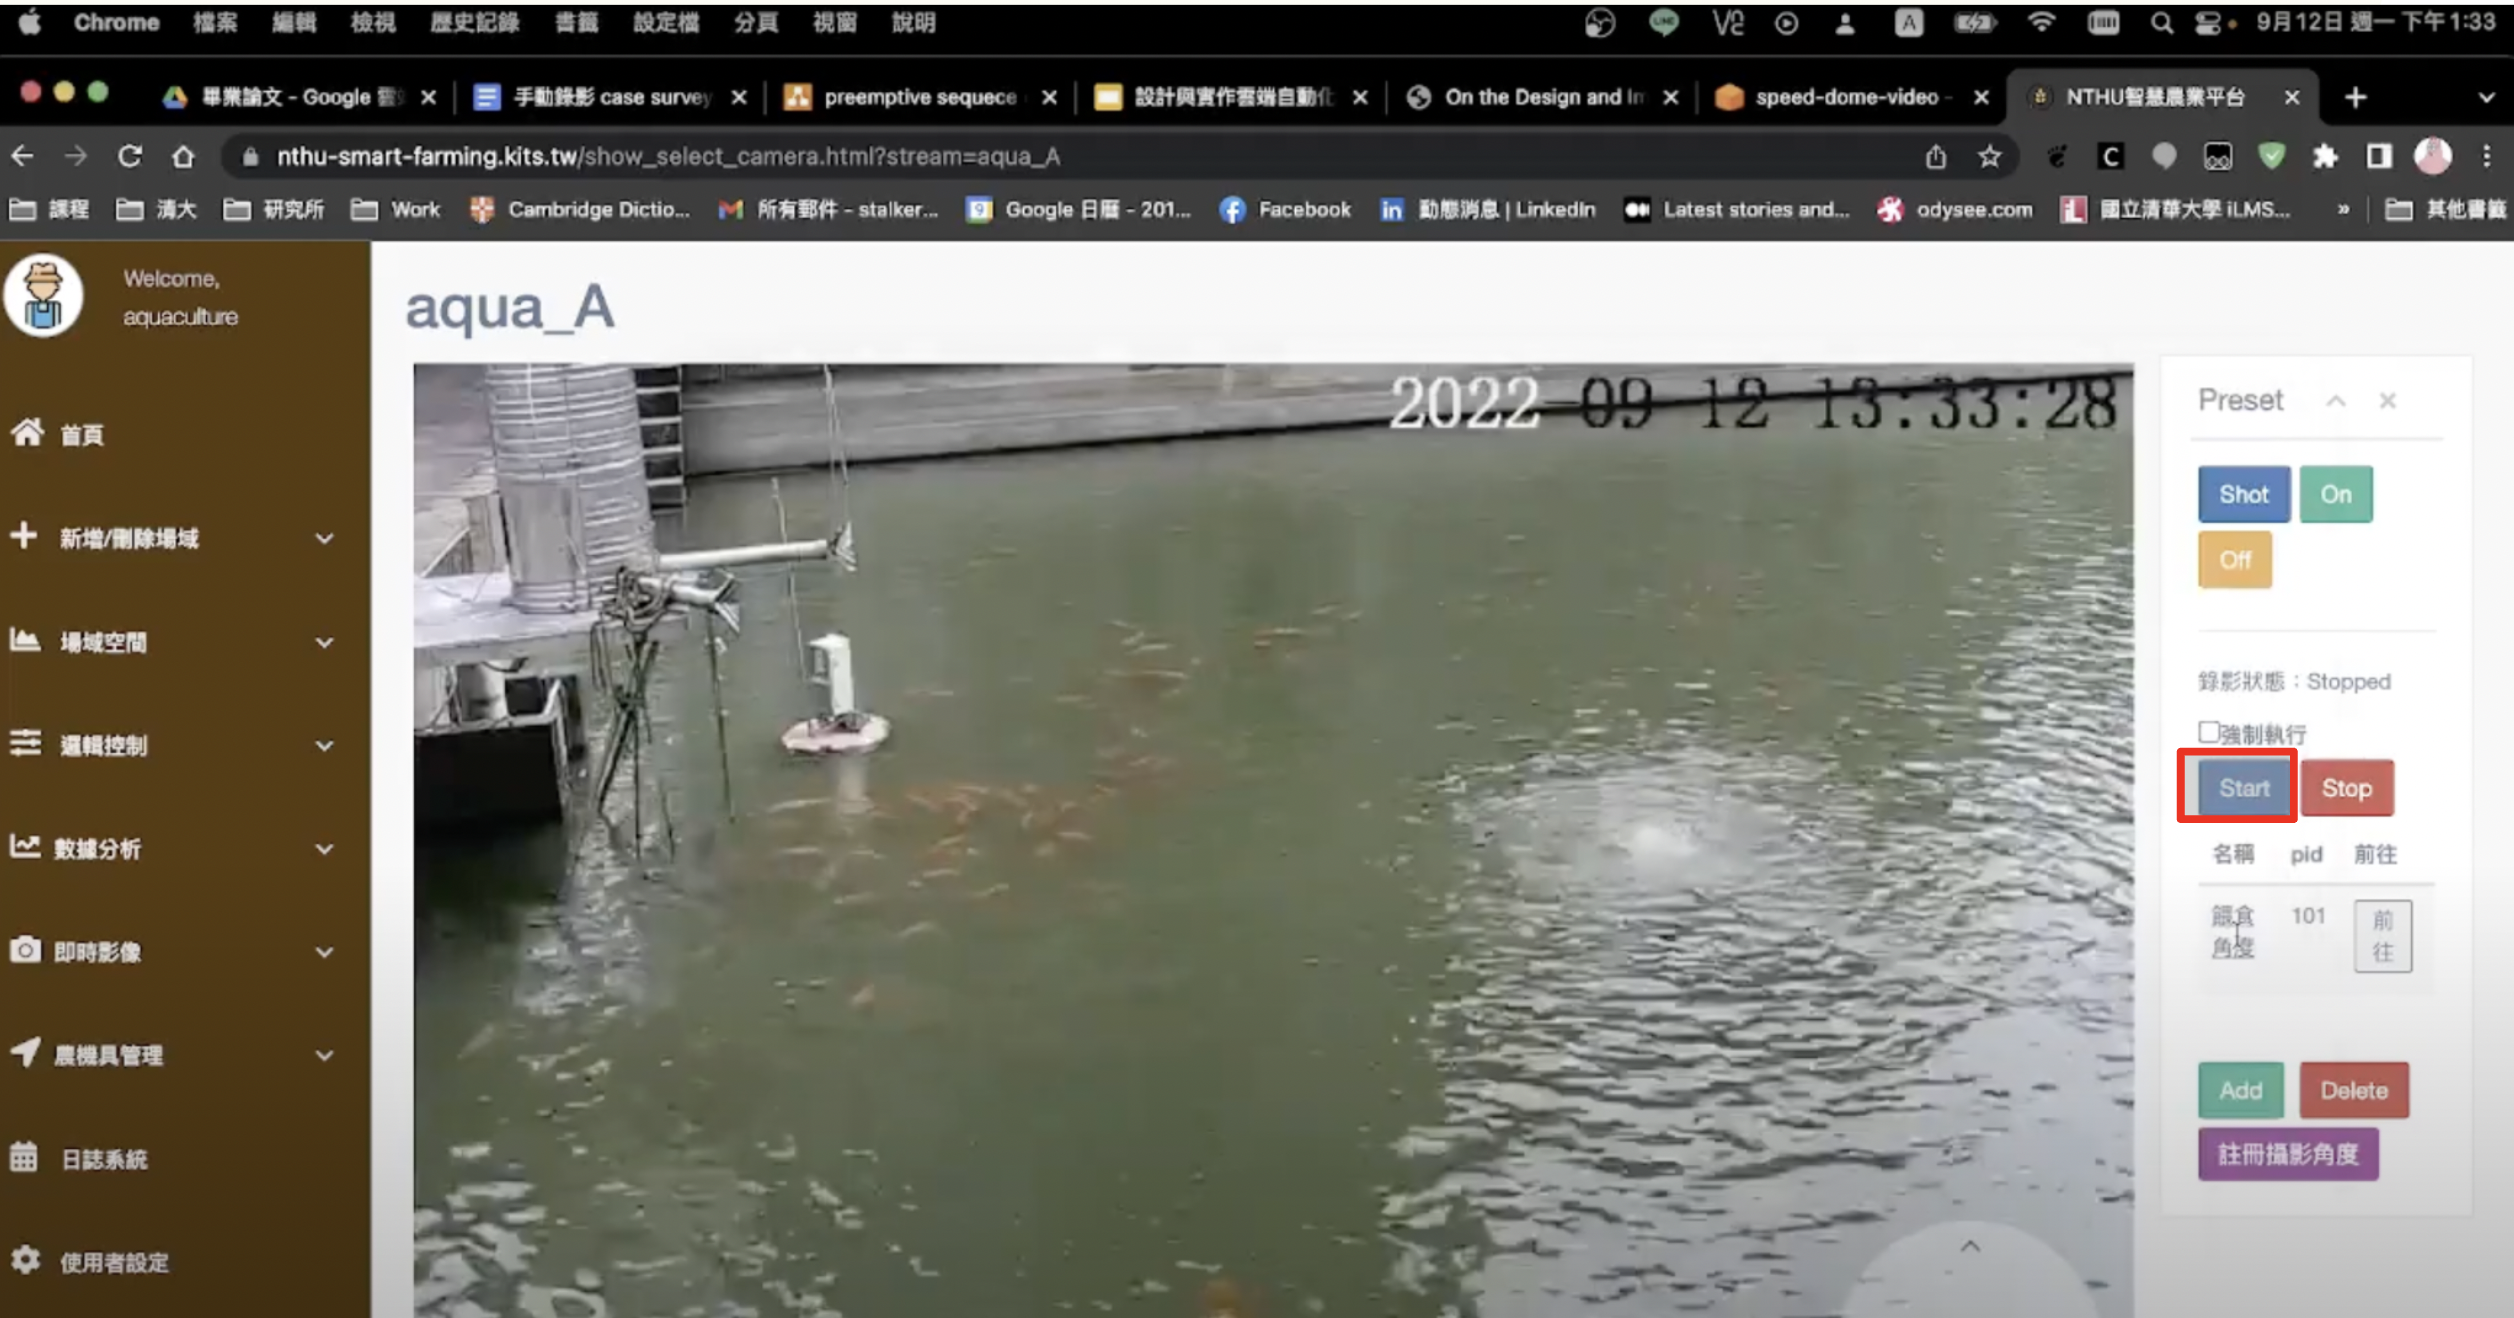
\includegraphics[width=\textwidth]{figsrc/demo-manual-1.png}
        \subcaption{Click start button}
        \label{fig:demo-manual-1}
    \end{subfigure}
\end{figure}

\begin{figure}[H]
    \ContinuedFloat
    \centering
    \begin{subfigure}{\textwidth}
        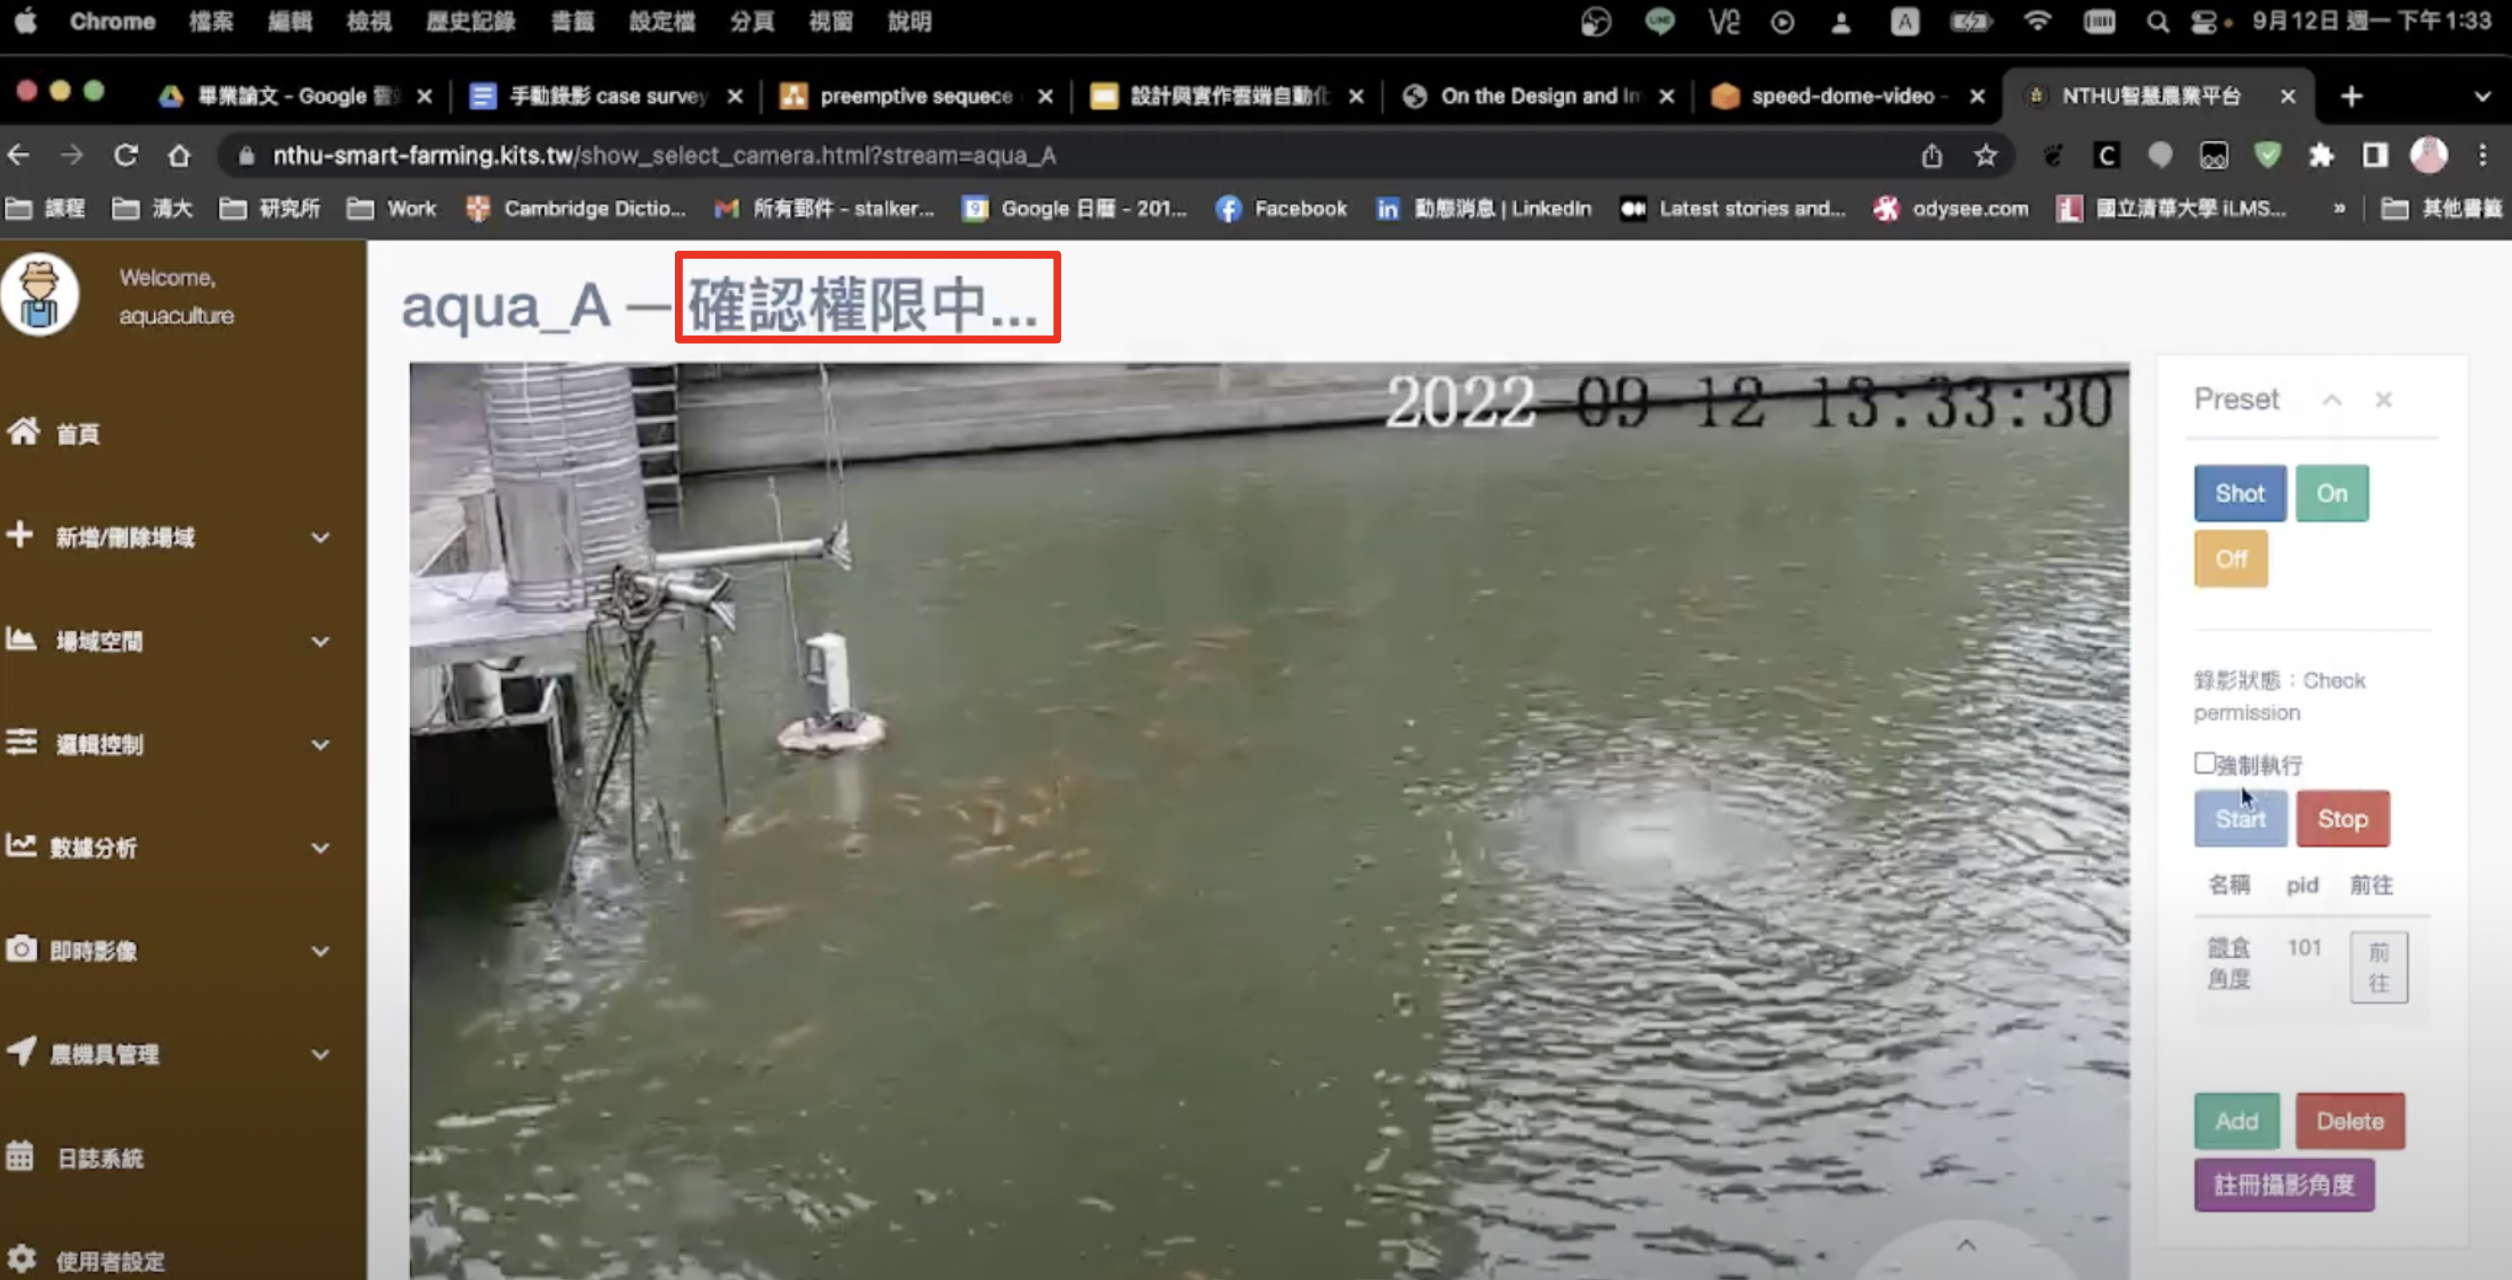
\includegraphics[width=\textwidth]{figsrc/demo-manual-2.png}
        \subcaption{Wait for permission}
        \label{fig:demo-manual-2}
    \end{subfigure}
\end{figure}

\begin{figure}[H]
    \ContinuedFloat
    \centering
    \begin{subfigure}{\textwidth}
        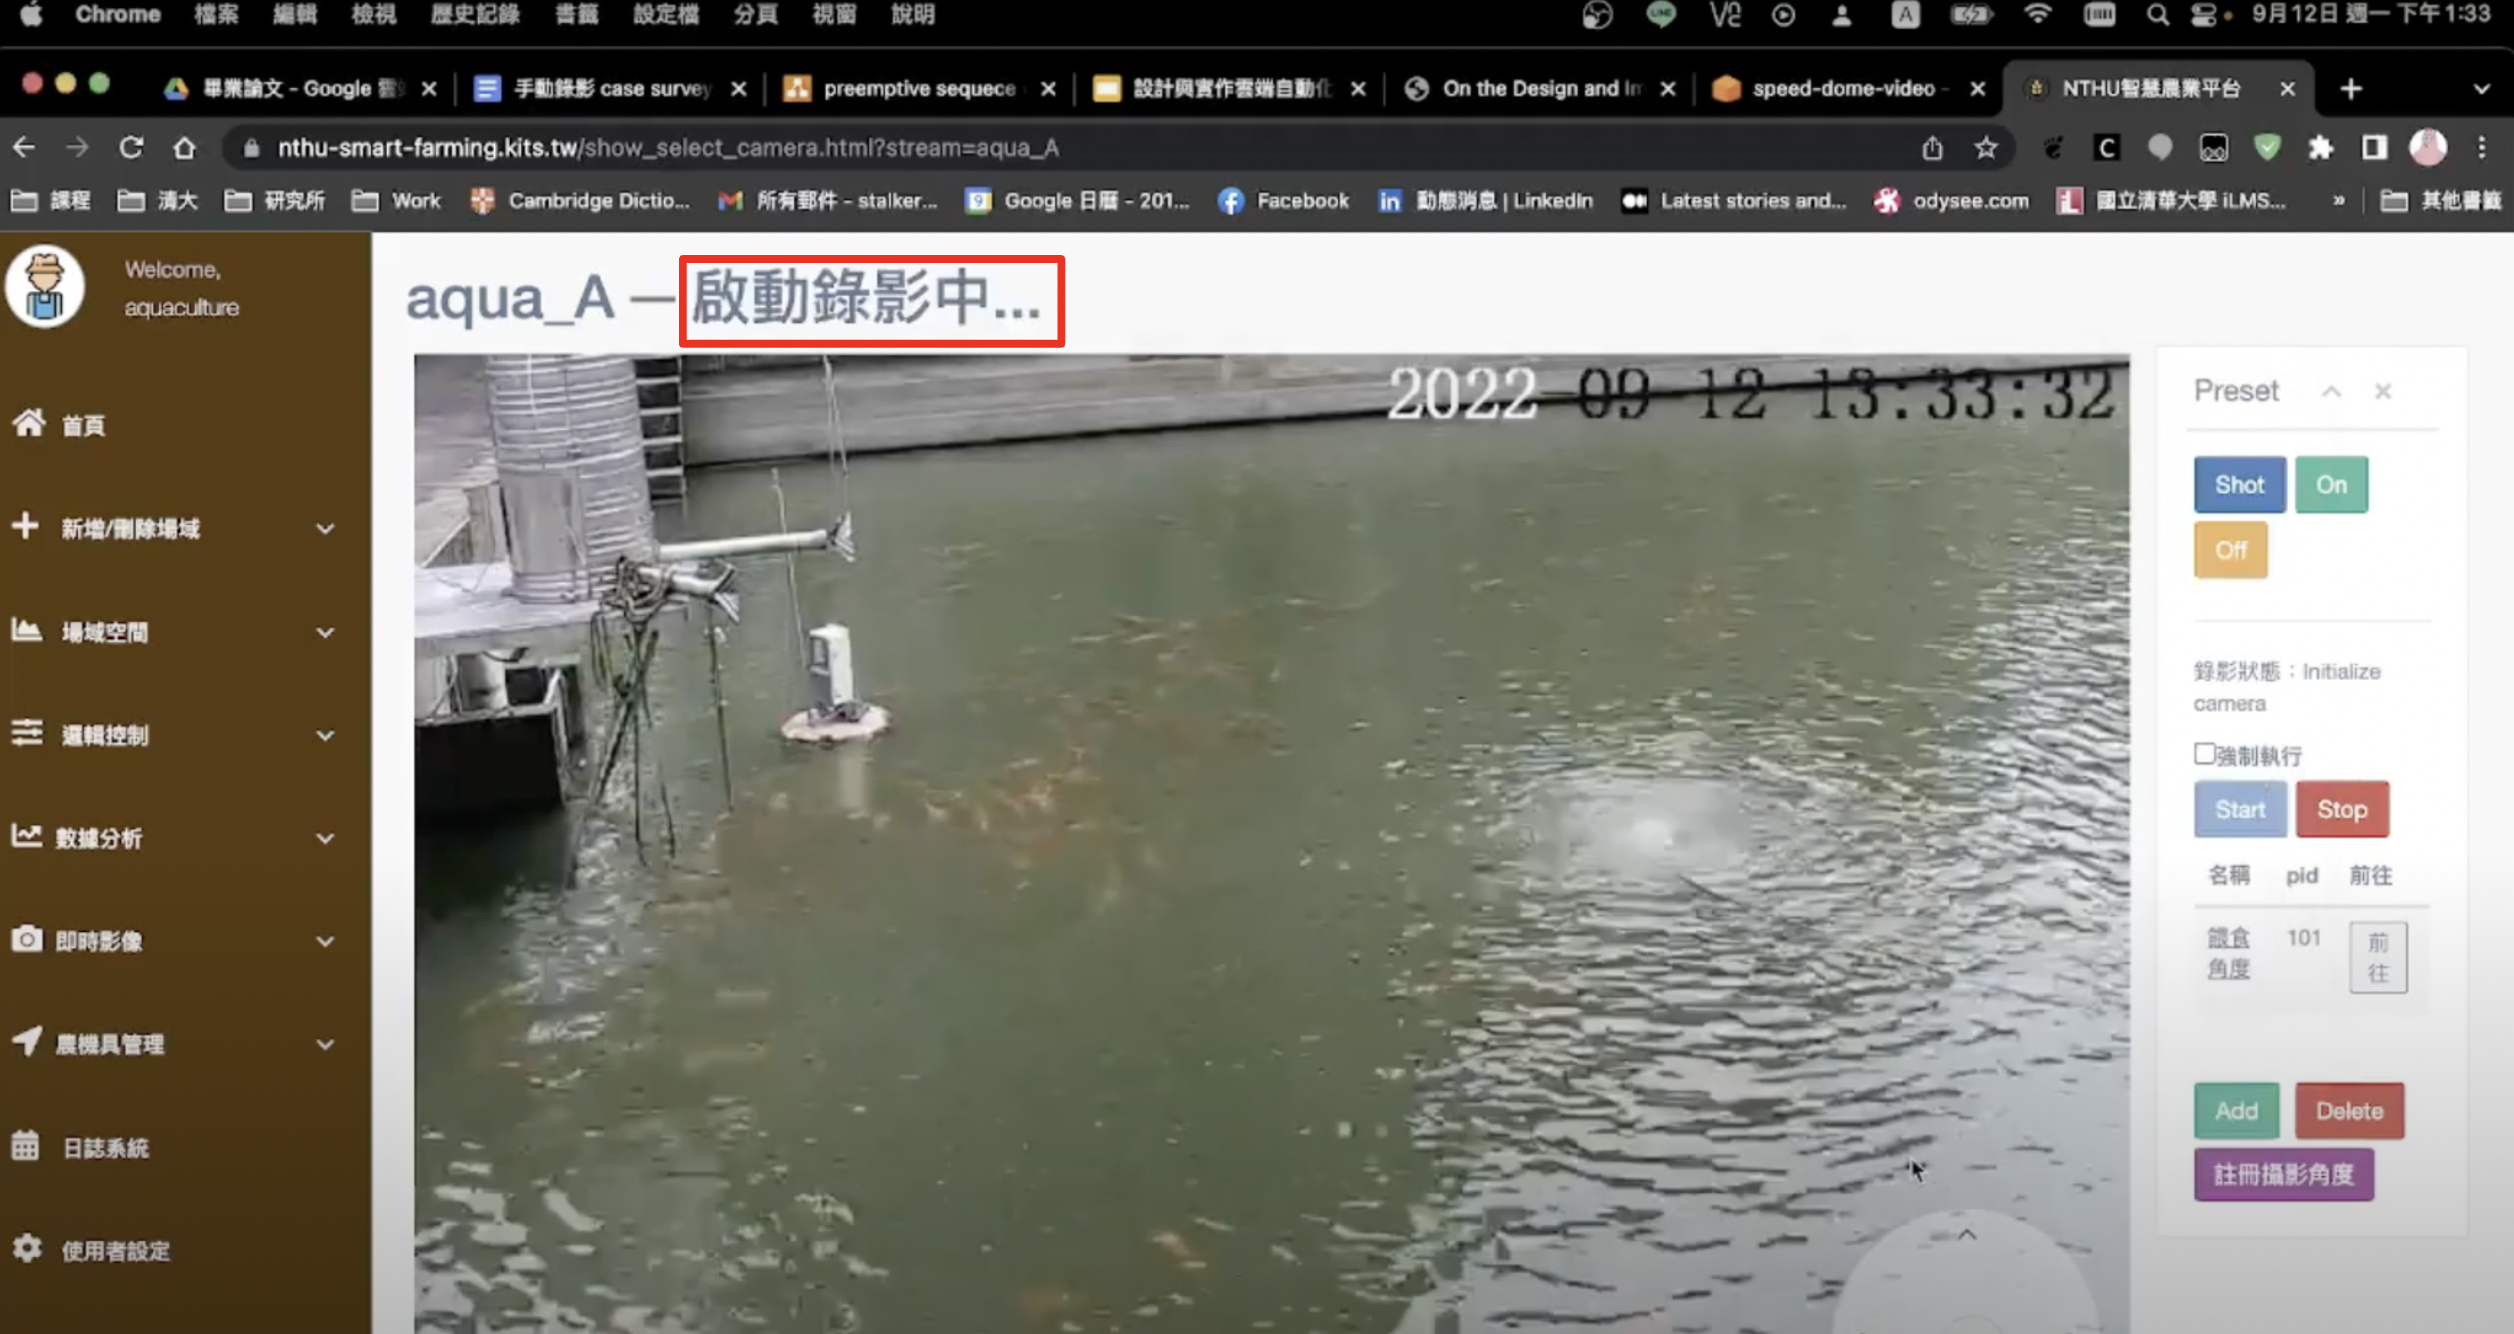
\includegraphics[width=\textwidth]{figsrc/demo-manual-3.png}
        \subcaption{Wait for connection}
        \label{fig:demo-manual-3}
    \end{subfigure}
\end{figure}

\begin{figure}[H]
    \ContinuedFloat
    \centering
    \begin{subfigure}{\textwidth}
        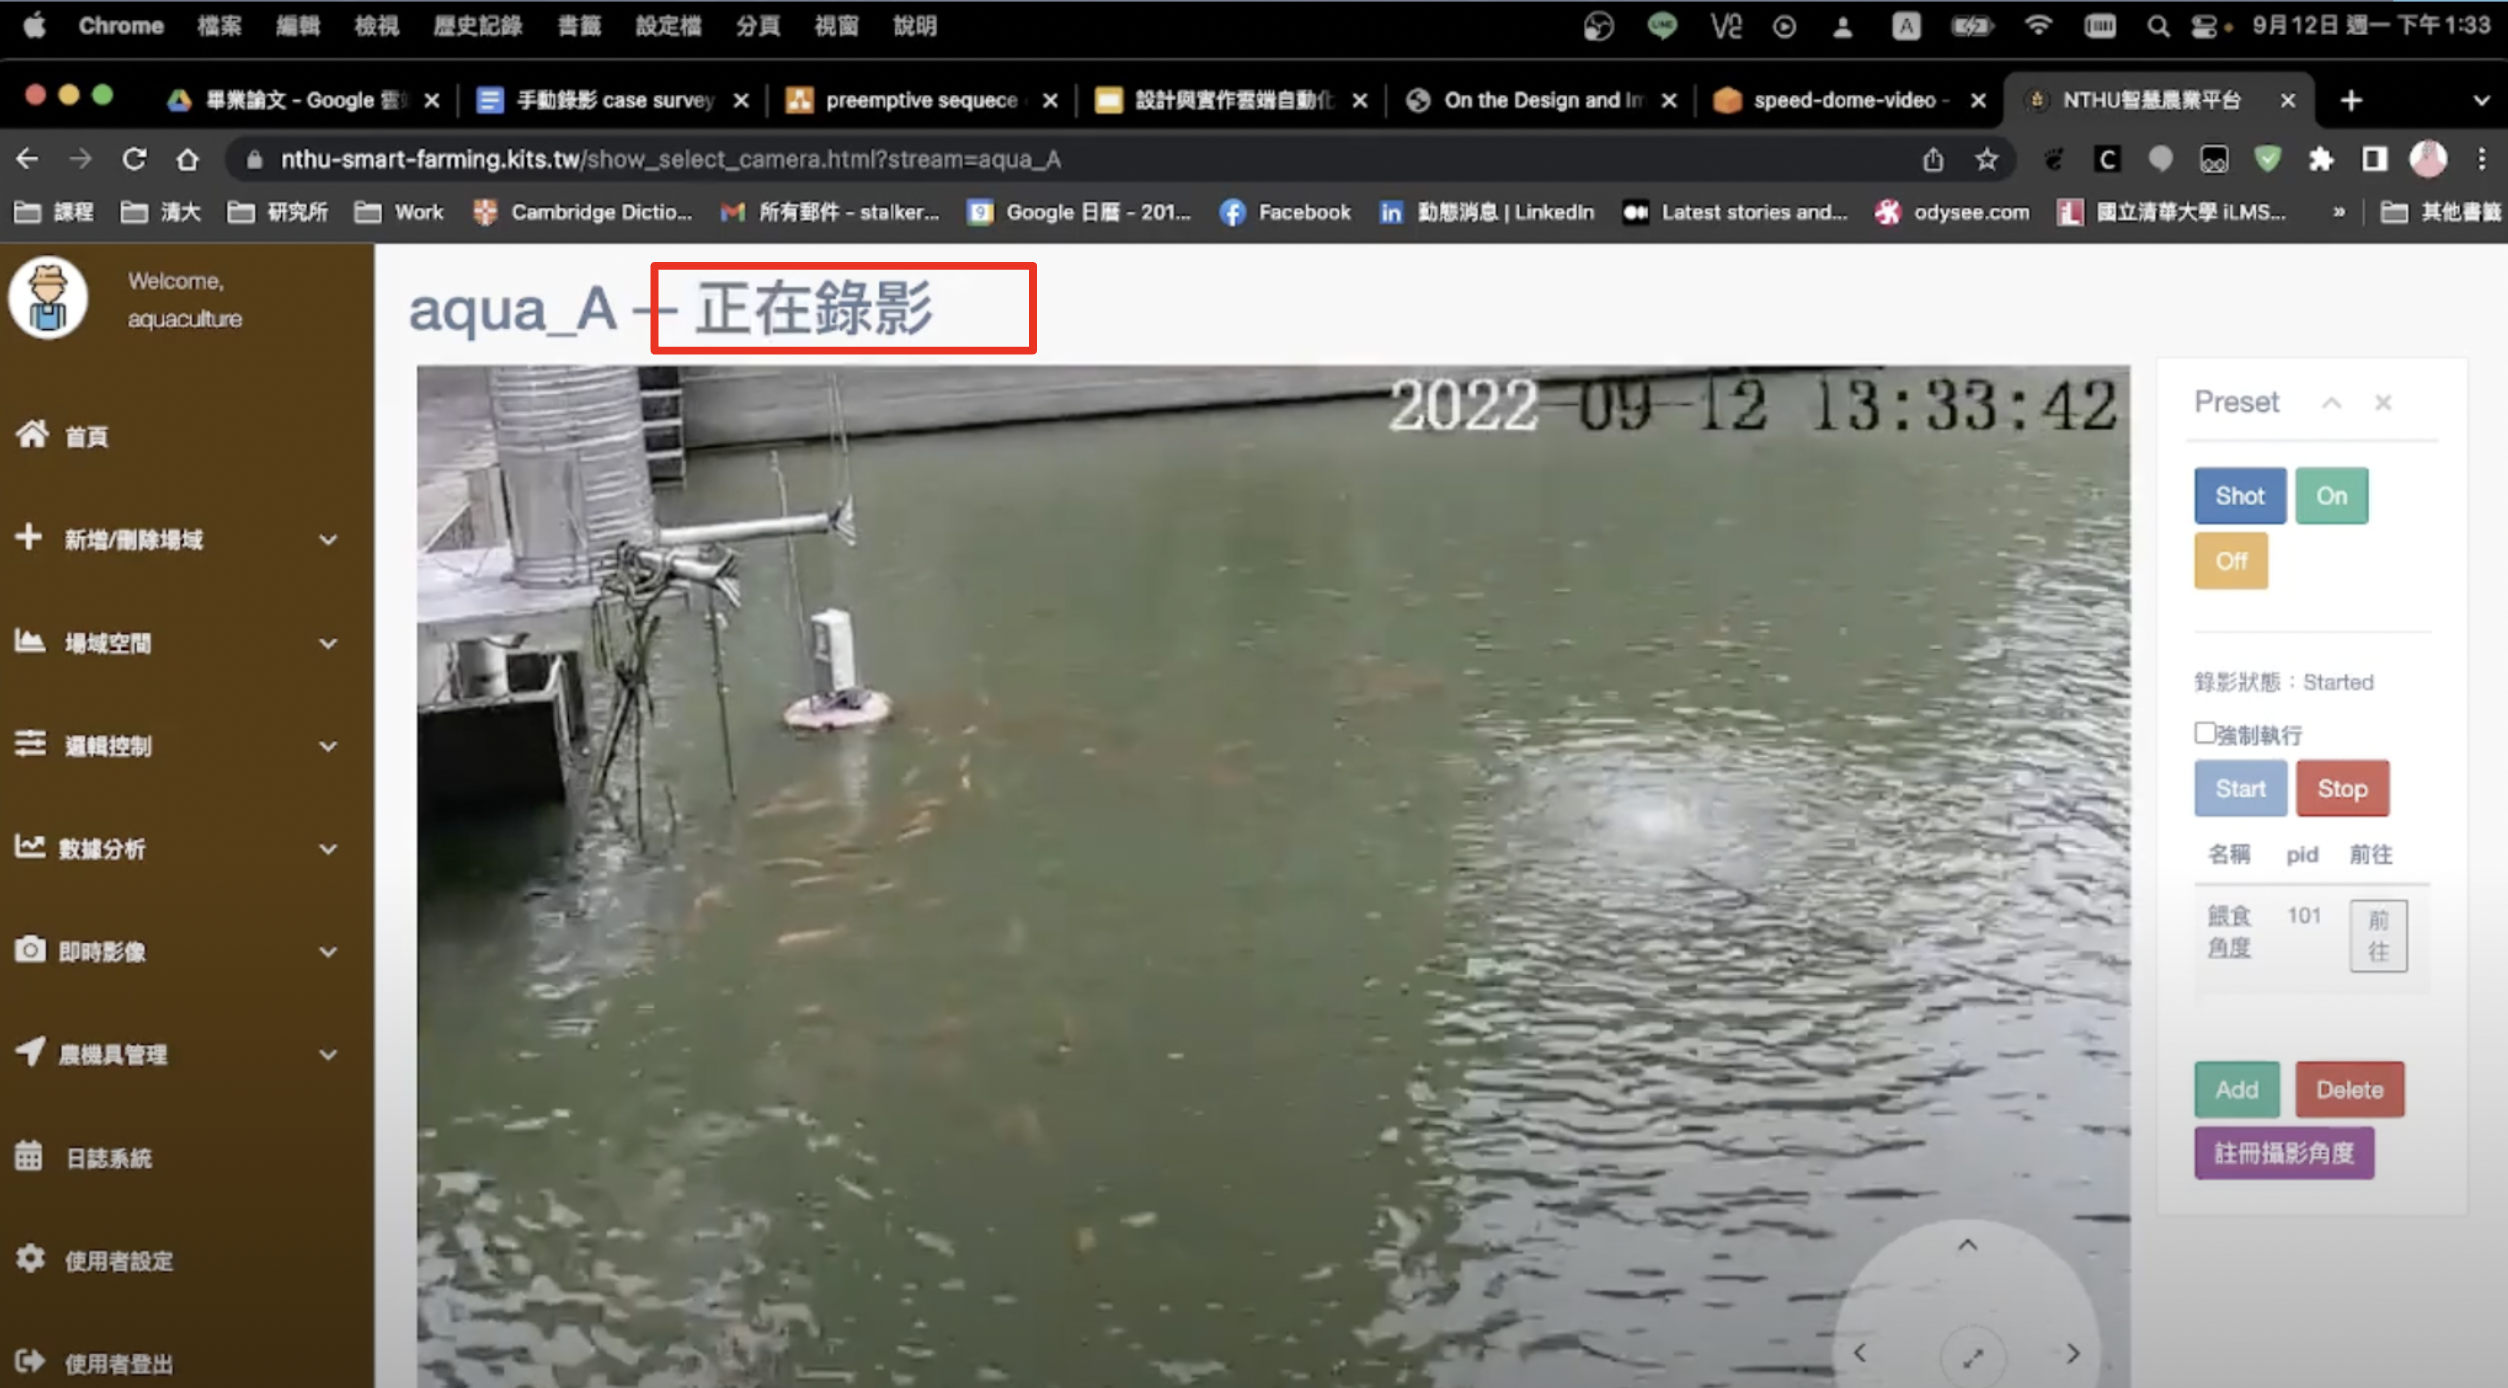
\includegraphics[width=\textwidth]{figsrc/demo-manual-4.png}
        \subcaption{Start recording}
        \label{fig:demo-manual-4}
    \end{subfigure}
\end{figure}


\begin{figure}[H]
    \ContinuedFloat
    \centering
    \begin{subfigure}{\textwidth}
        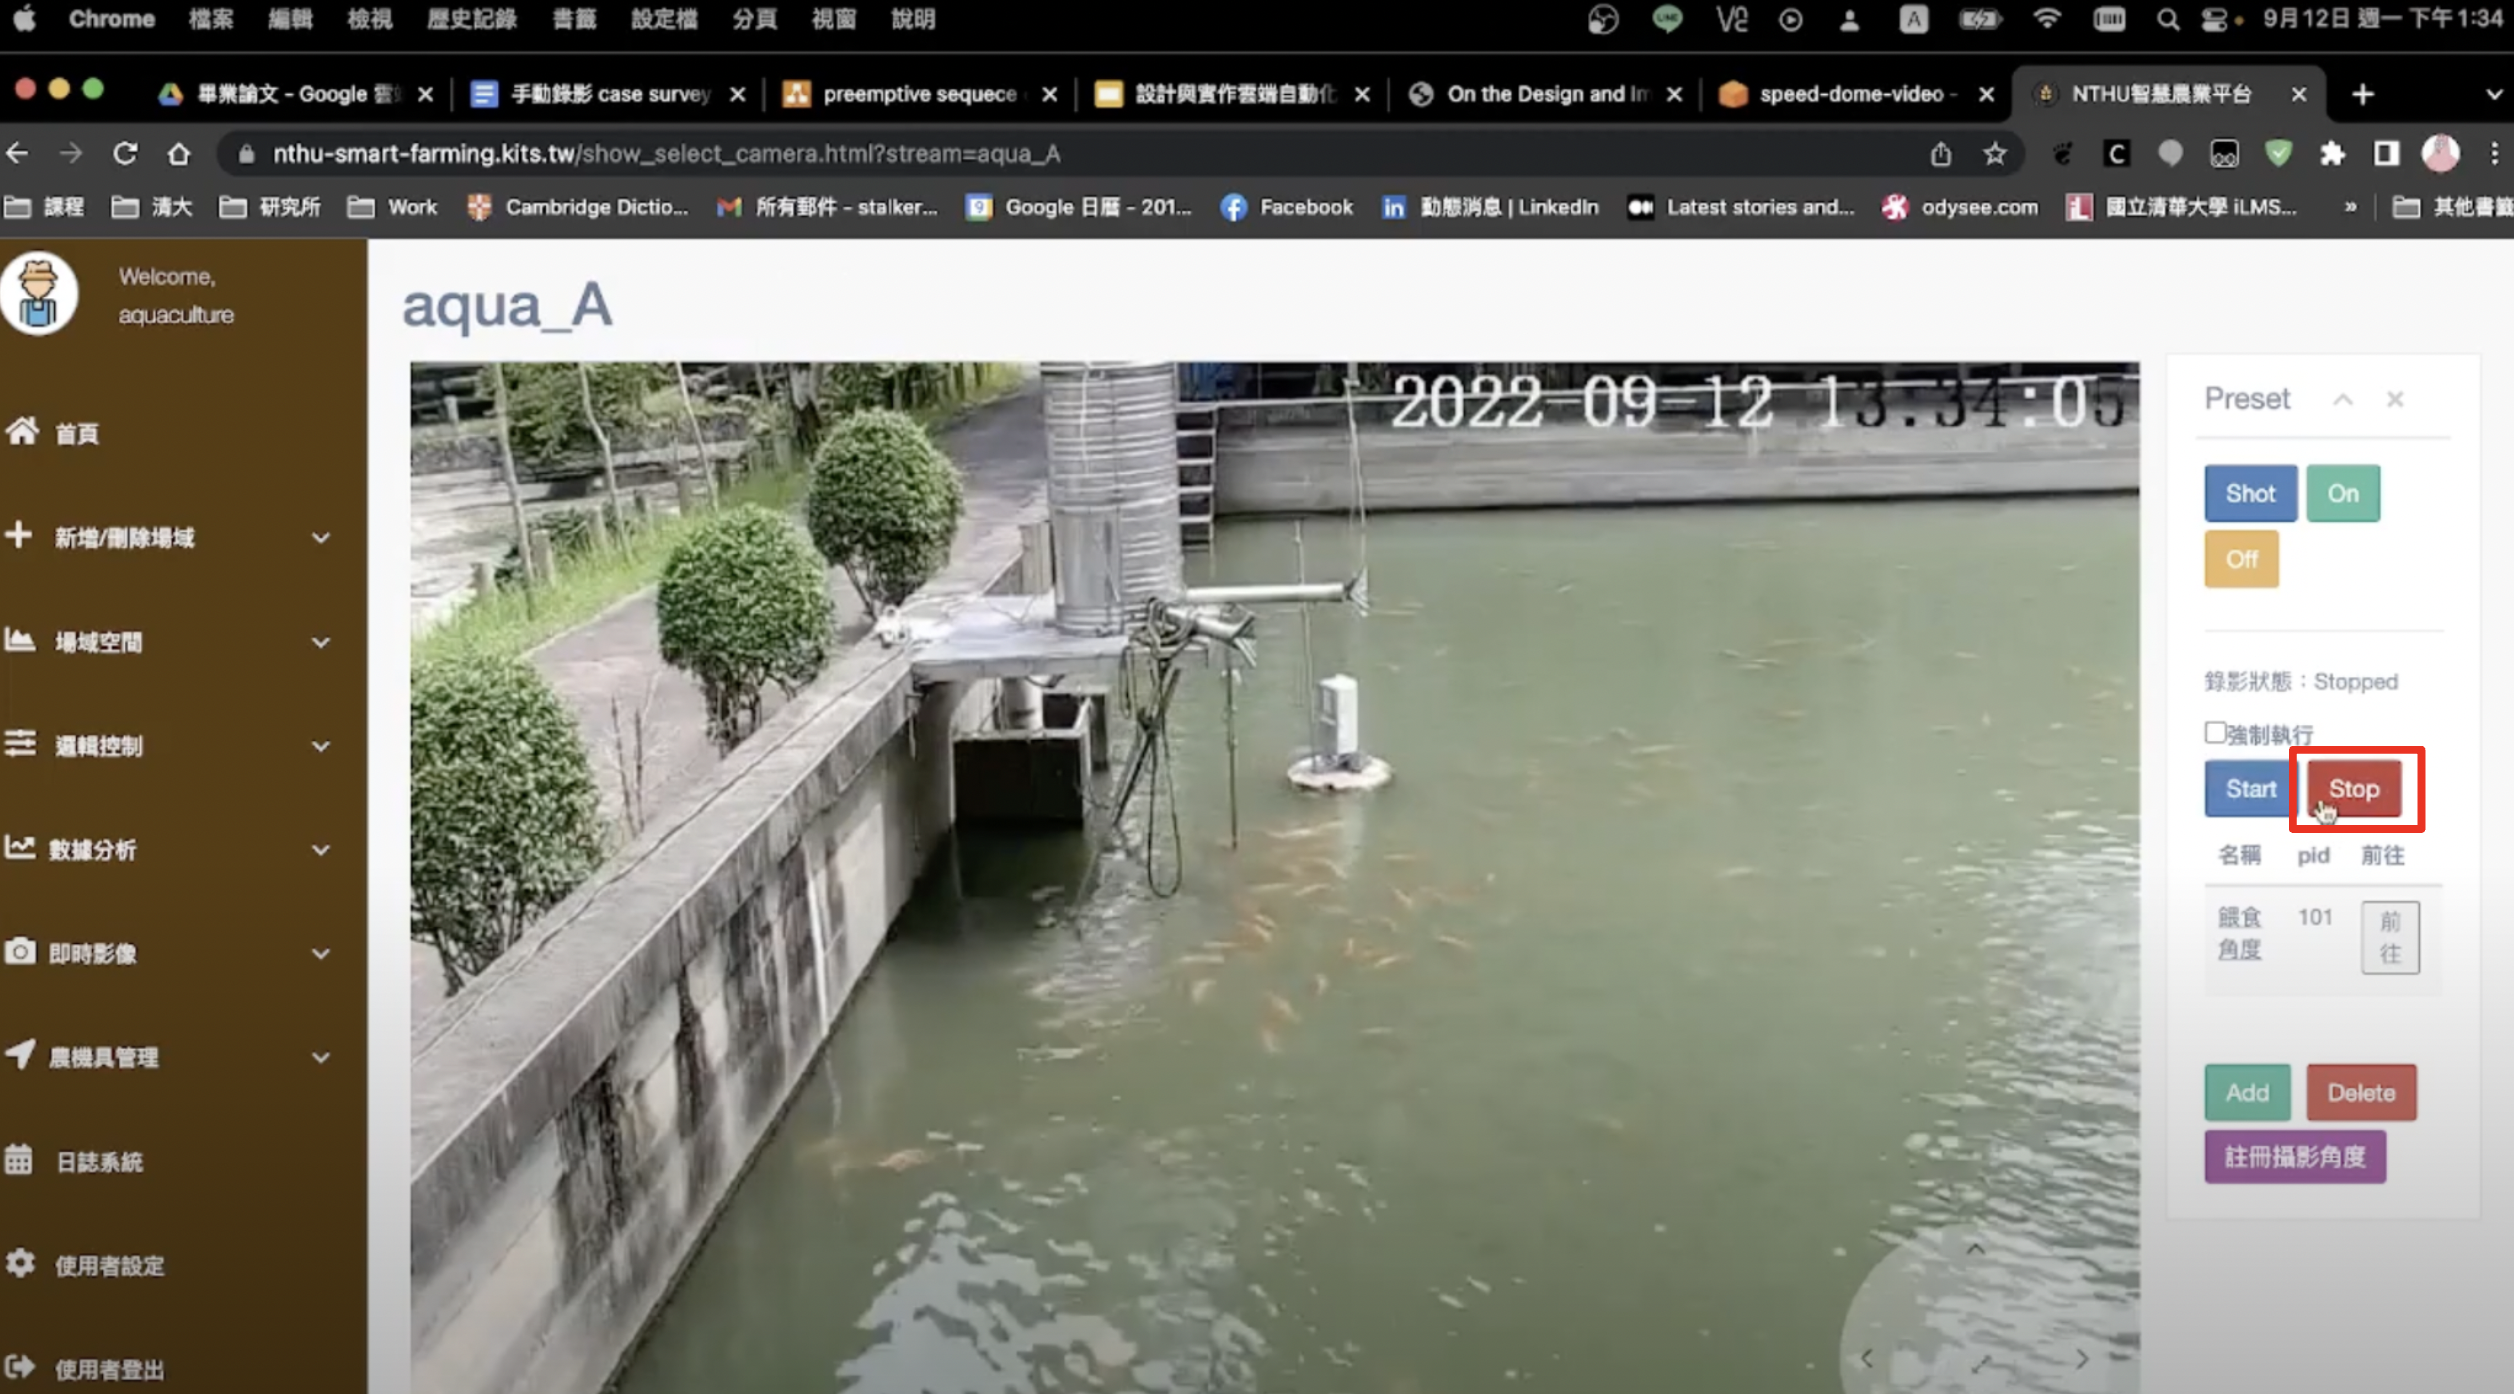
\includegraphics[width=\textwidth]{figsrc/demo-manual-5.png}
        \subcaption{Stop recording}
        \label{fig:demo-manual-5}
    \end{subfigure}

    \caption{DEMO of manual case}
    \label{fig:demo-manual}
\end{figure}

% time triggered(event trigger那邊平台還沒做好)
\subsection{Triggered based record}
Video DEMO: https://www.youtube.com/watch?v=yN4NbbG5he4

We will show the situation of sequence diagram of Fig.~\ref{fig:time-sequence-diagram} that happened in Front-end. We first set, duration, angle and the timing to record at 1:39PM, one minute later in Fig.~\ref{fig:demo-time-1}. At this moment, Scheduling server will recieve new setting that waits to execute. When time's up, scheduling server will reuqest PI to record. PI turns the camera from Fig.~\ref{fig:demo-time-2} to Fig.~\ref{fig:demo-time-3} at video timestamp 1:00\~1:05 then orders recording server to start the process.

\begin{figure}[H]
    \centering
    \begin{subfigure}{\textwidth}
        \includegraphics[width=\textwidth]{figsrc/demo-time-1.png}
        \subcaption{Set time schedule}
        \label{fig:demo-time-1}
    \end{subfigure}
\end{figure}


\begin{figure}[H]
    \ContinuedFloat
    \centering
    \begin{subfigure}{\textwidth}
        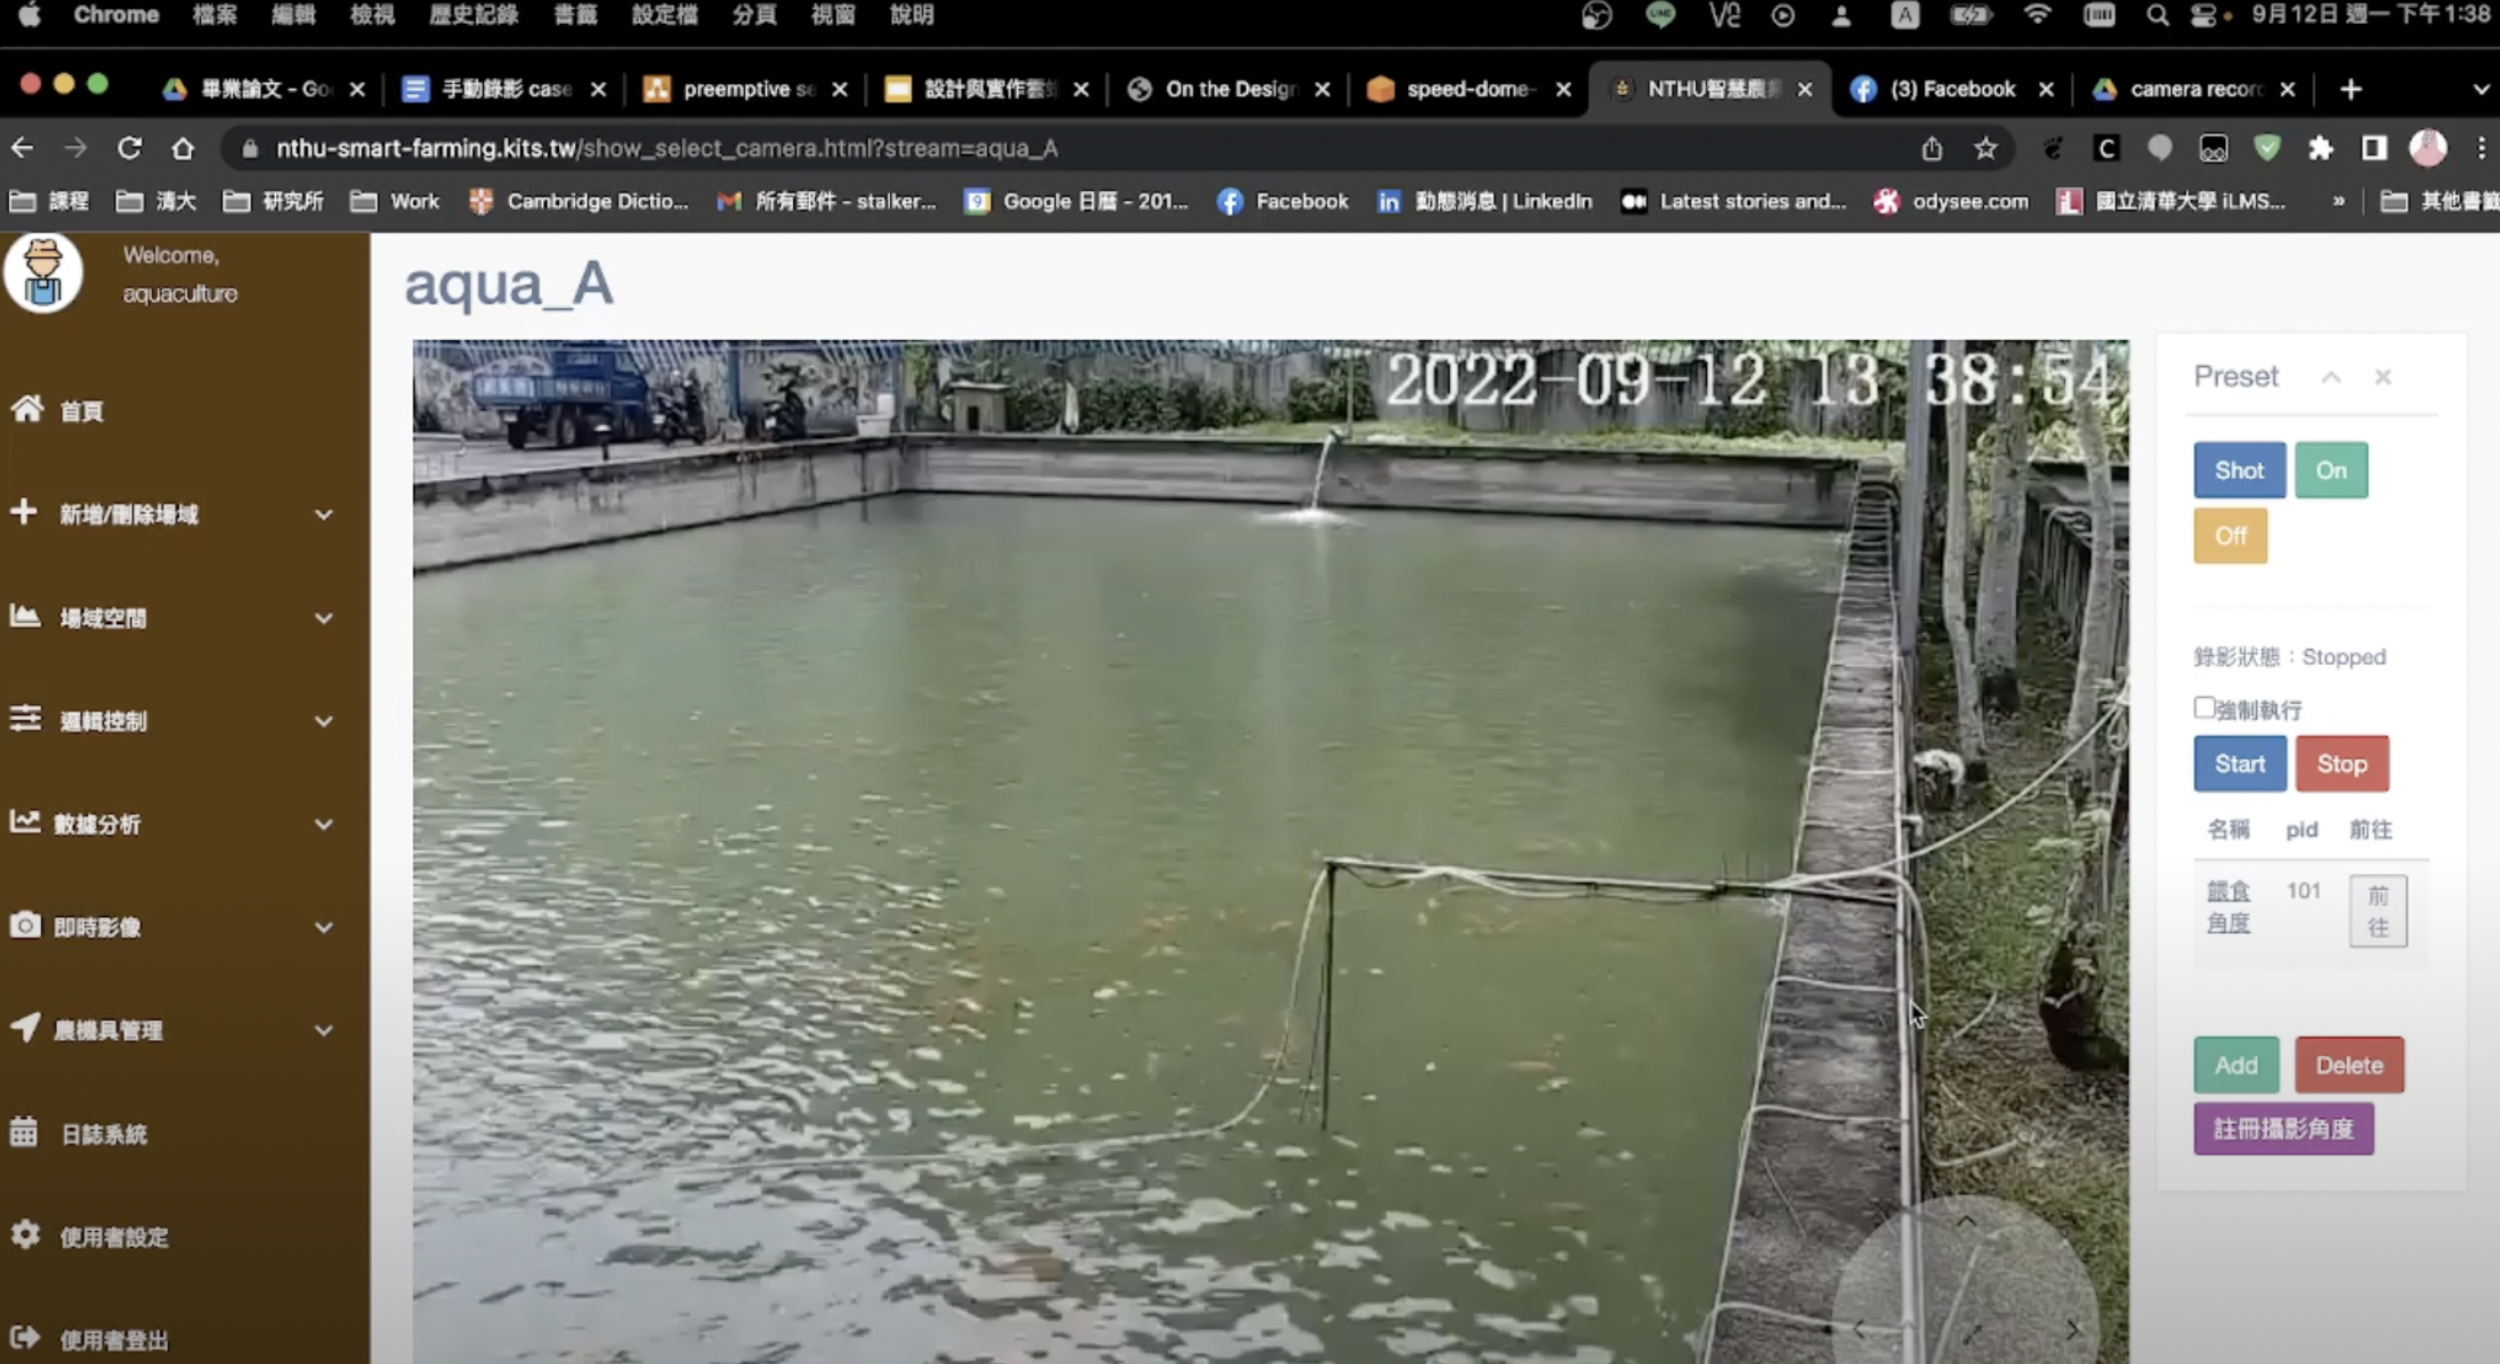
\includegraphics[width=\textwidth]{figsrc/demo-time-2.png}
        \subcaption{Angle before recording}
        \label{fig:demo-time-2}
    \end{subfigure}
\end{figure}

\begin{figure}[H]
    \ContinuedFloat
    \centering
    \begin{subfigure}{\textwidth}
        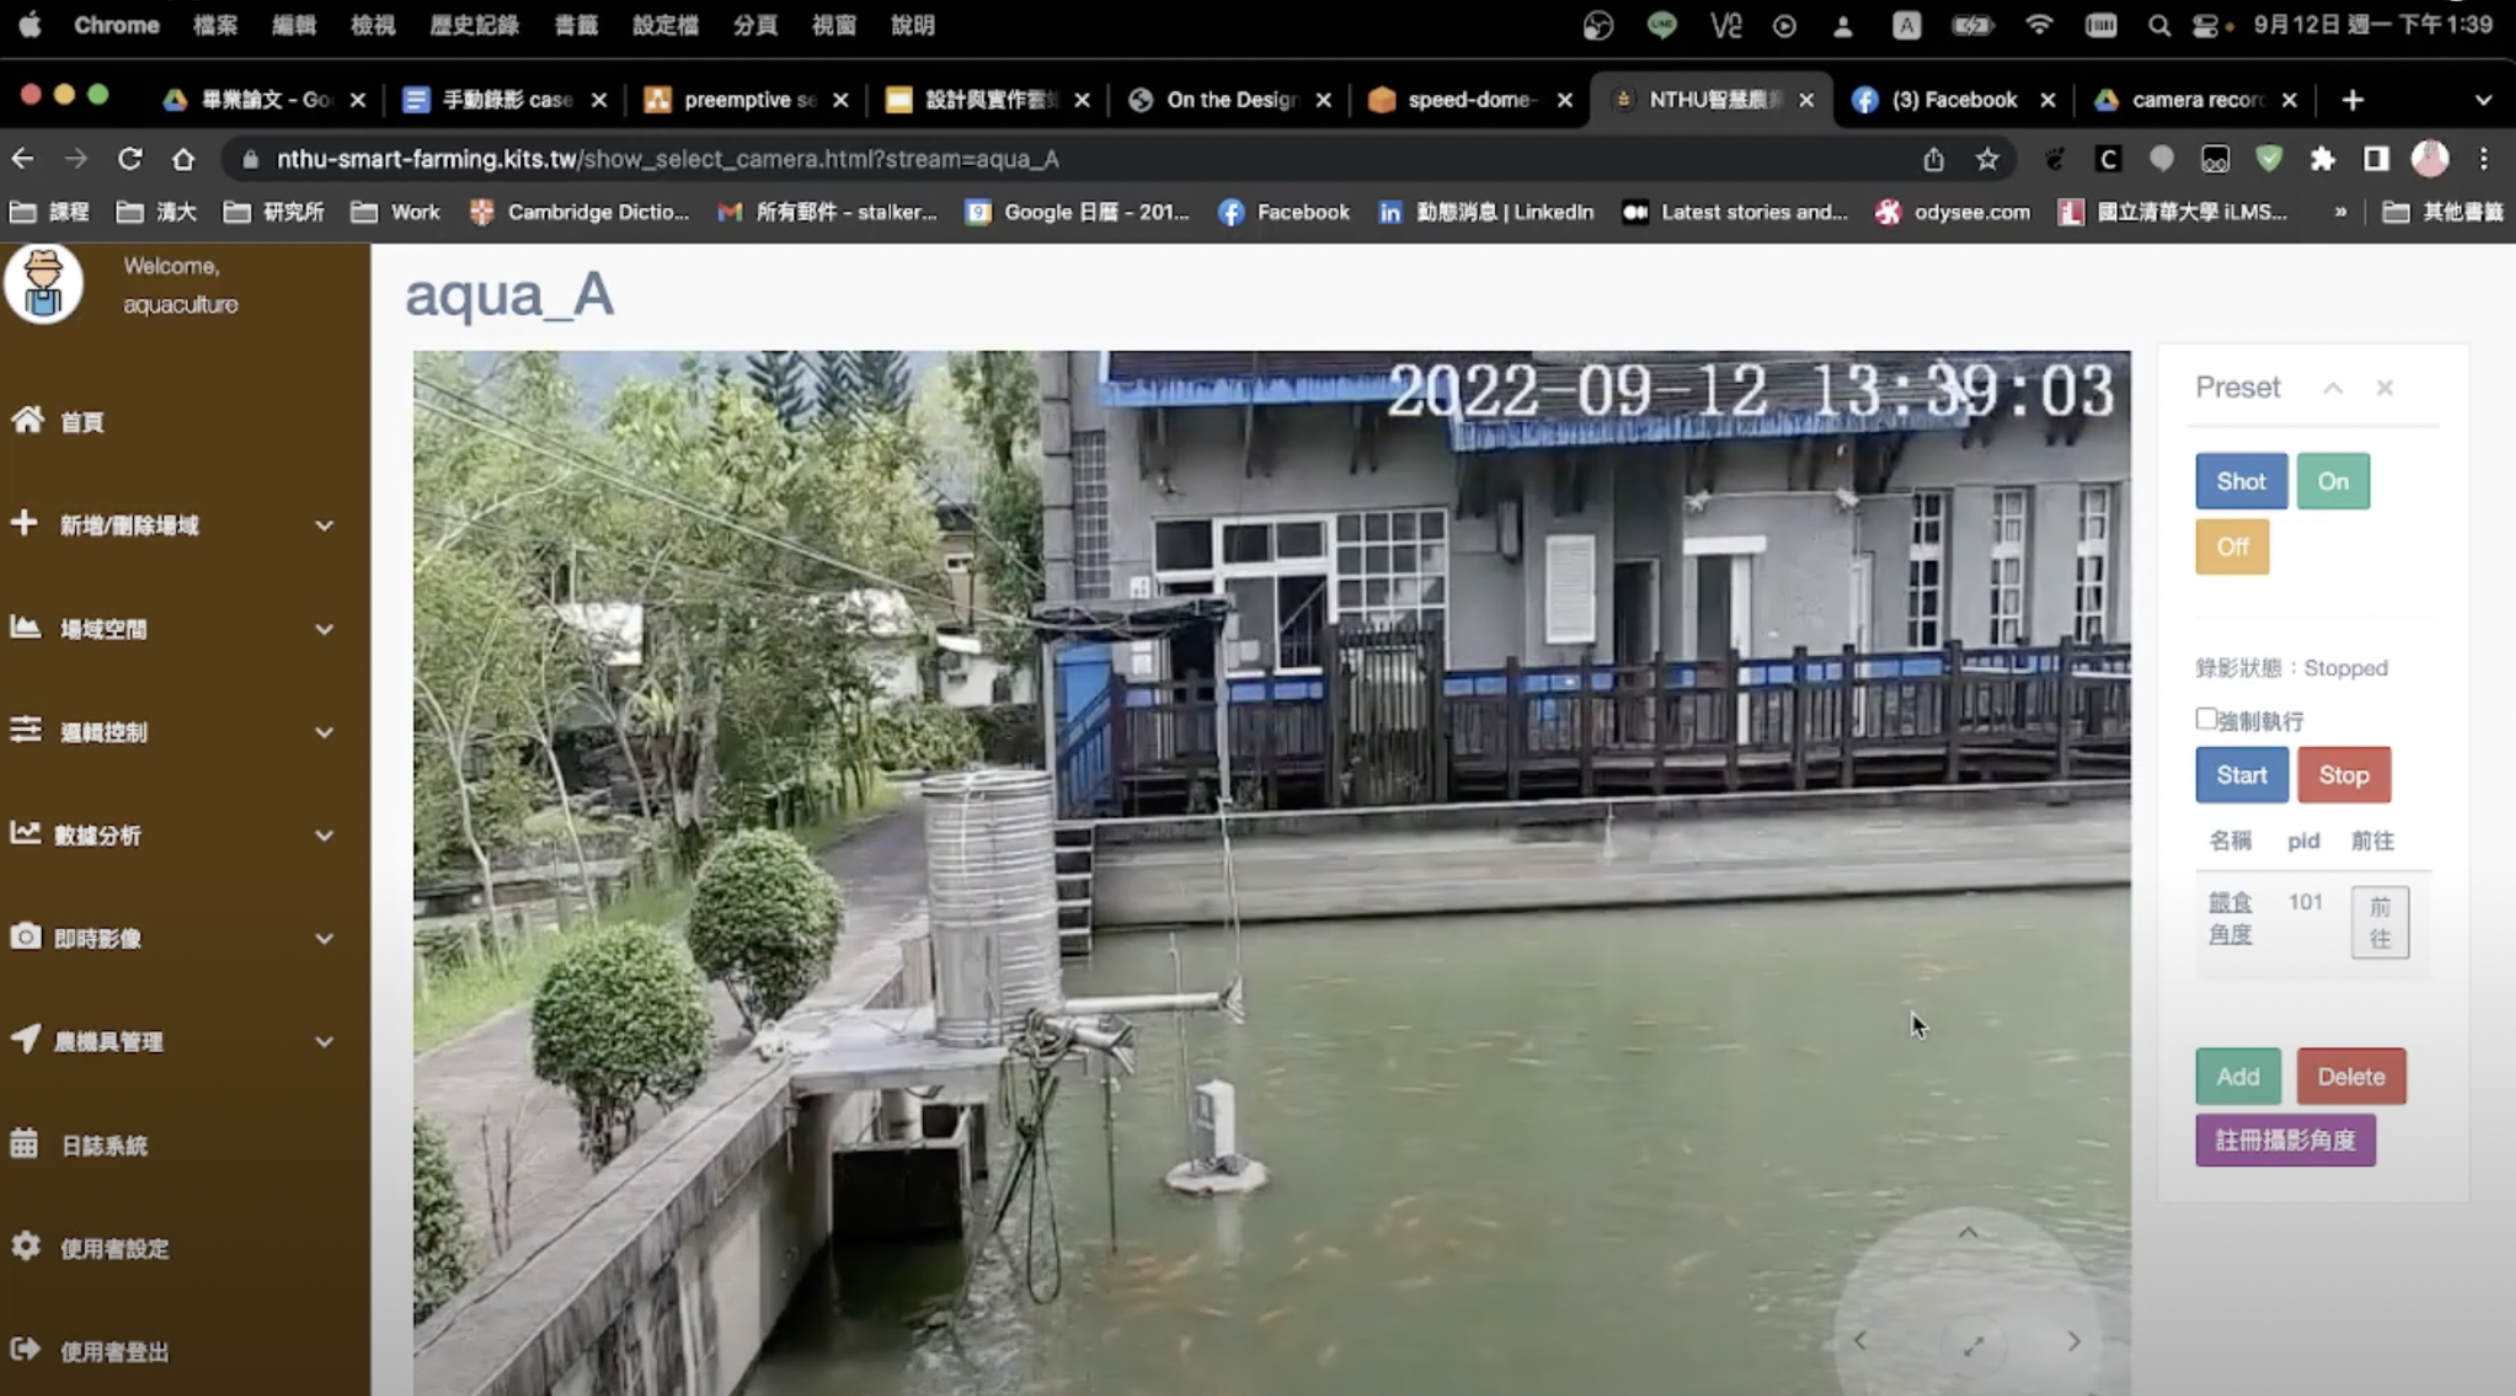
\includegraphics[width=\textwidth]{figsrc/demo-time-3.png}
        \subcaption{Angle after recording}
        \label{fig:demo-time-3}
    \end{subfigure}

    \caption{DEMO of triggered case}
    \label{fig:demo-time}
\end{figure}

% higher preemptive
\subsection{Higher preemptive case}
Video DEMO: https://www.youtube.com/watch?v=\_GLhjjII8Pg

We will show how higher priority task preempt lower priority one in Front-end side. As shown in Fig~\ref{fig:demo-higher-1}, we first set a request that will occur one minute later, then we start manual record in Fig.~\ref{fig:demo-higher-2}. In Fig.~\ref{fig:demo-higher-3}, When time request triggers, we can see in web page that it will stop the recording preocess and send alert to user. At the same time, recording server will upload user's video file to AWS S3 then start new recording task. The preemptive data flow can be saw in Chapter 3 Fig.\ref{fig:preemptive-B-higher}.


\begin{figure}[H]
    \centering
    \begin{subfigure}{\textwidth}
        \includegraphics[width=\textwidth]{figsrc/demo-higher-1.png}
        \subcaption{Set time schedule}
        \label{fig:demo-higher-1}
    \end{subfigure}
\end{figure}

\begin{figure}[H]
    \ContinuedFloat
    \centering
    \begin{subfigure}{\textwidth}
        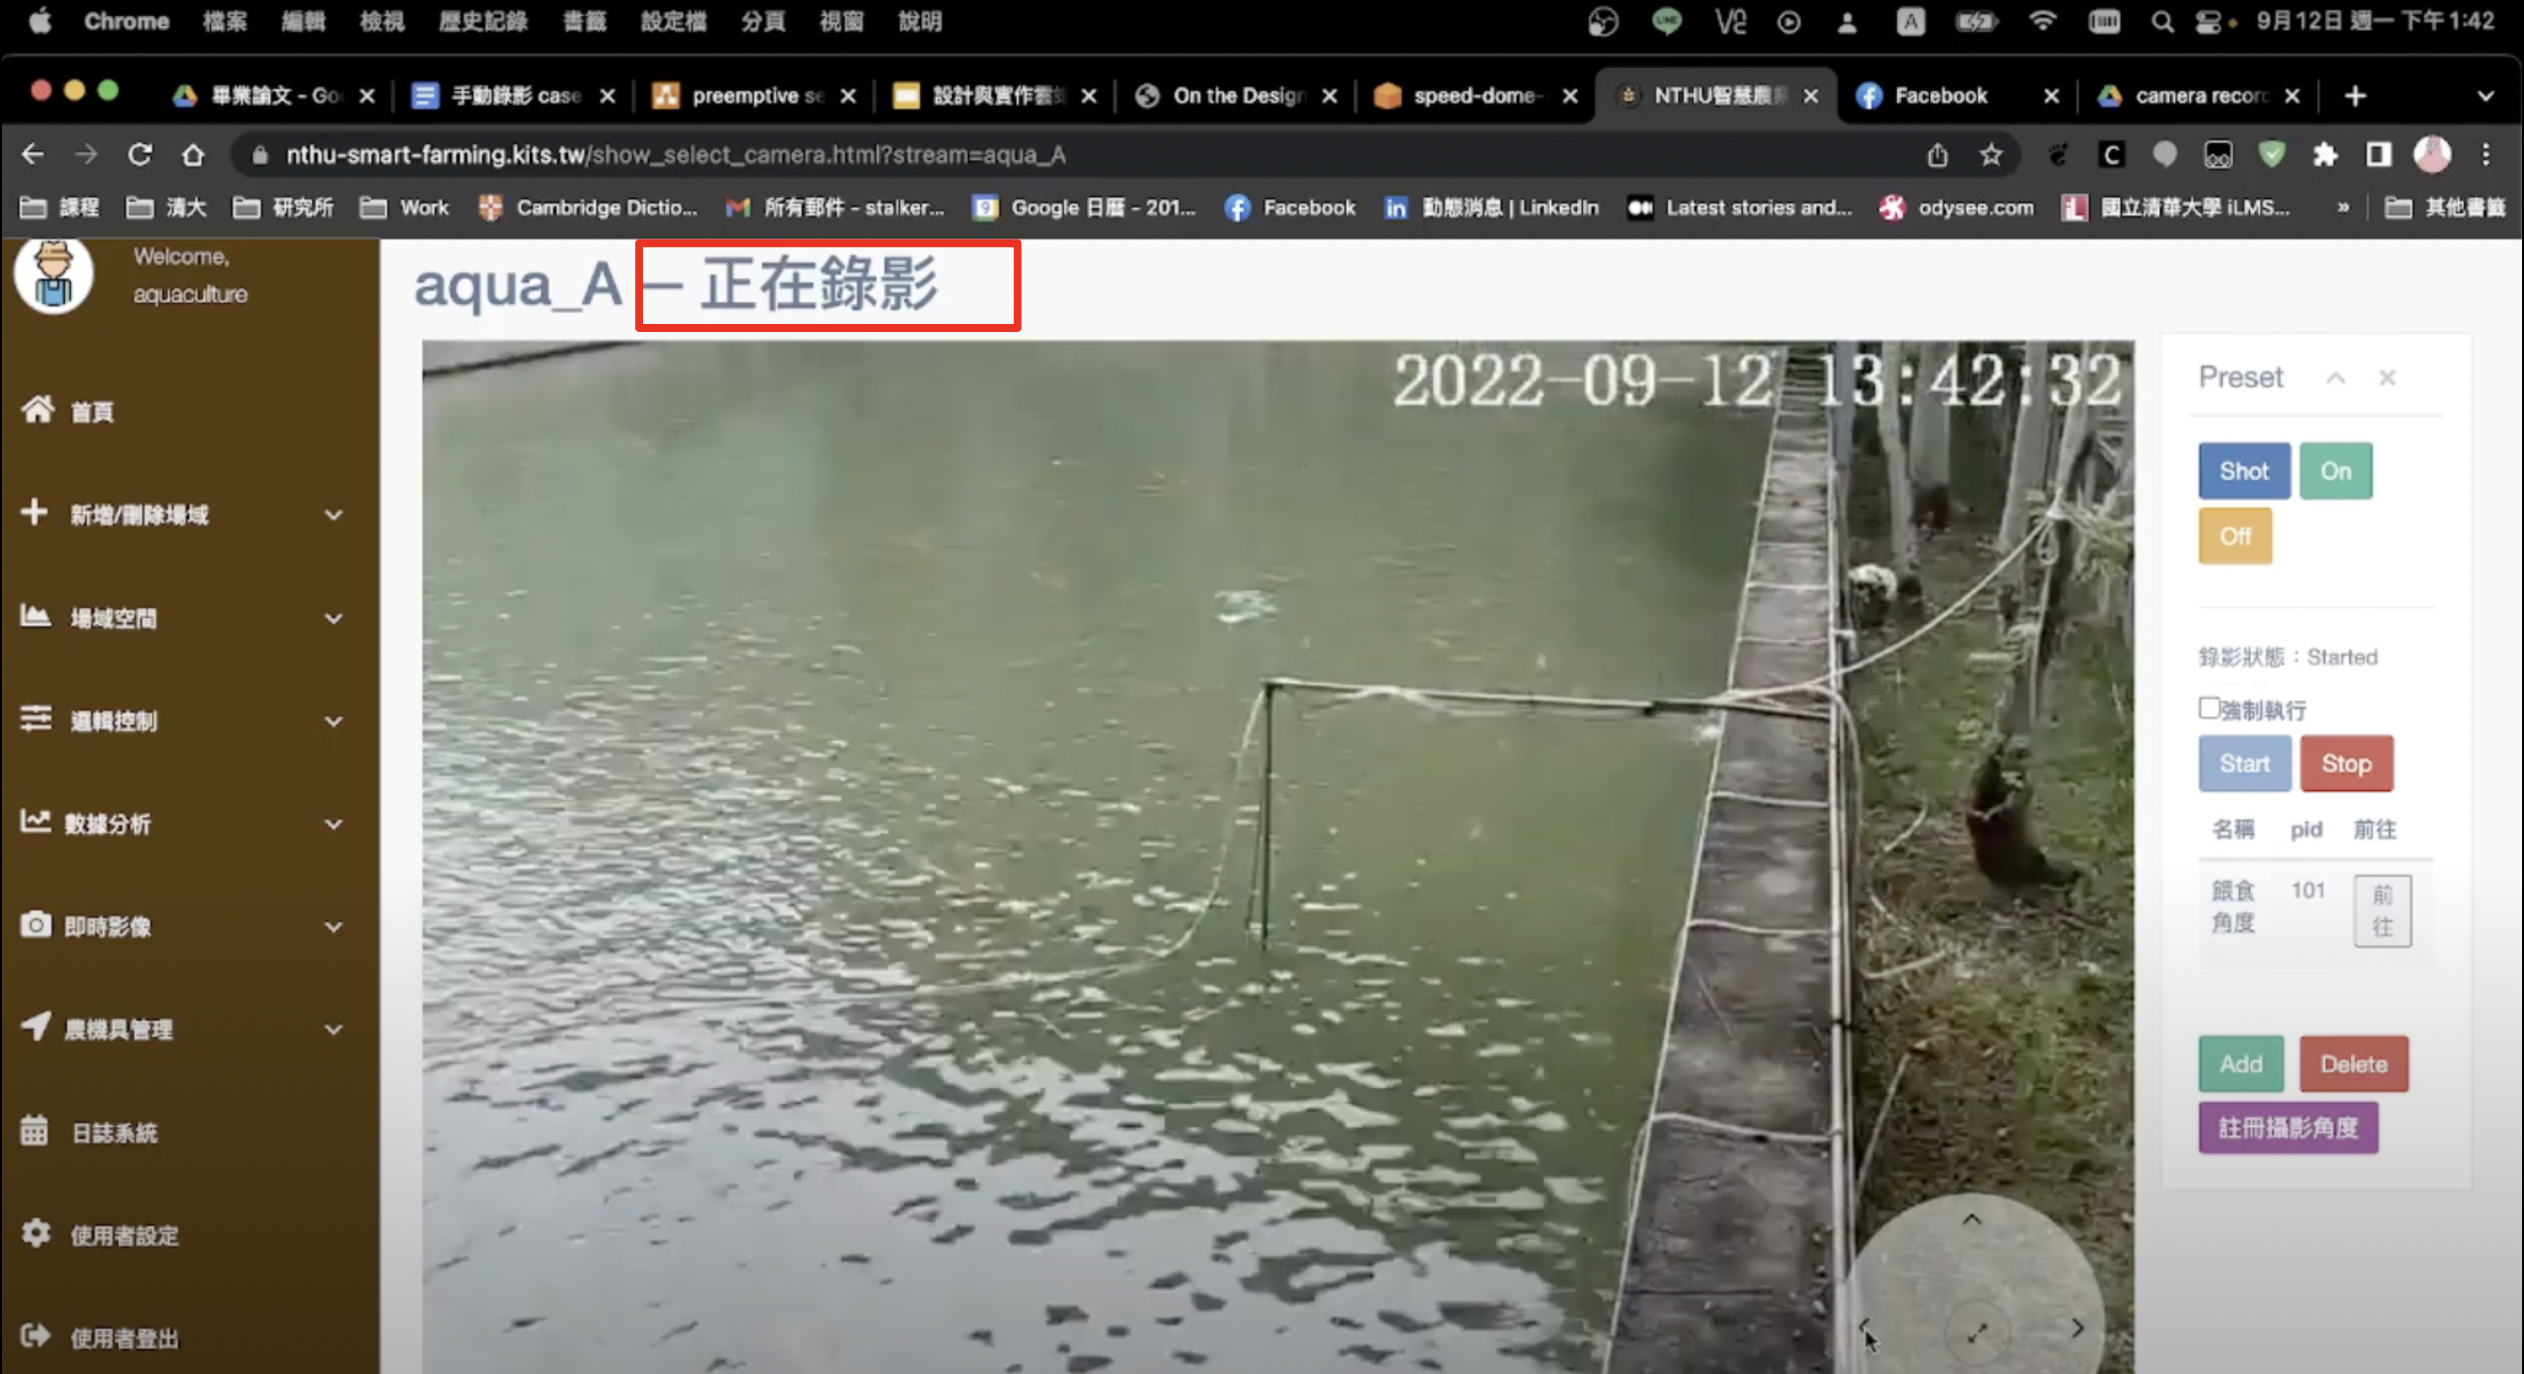
\includegraphics[width=\textwidth]{figsrc/demo-higher-2.png}
        \subcaption{Start manual record}
        \label{fig:demo-higher-2}
    \end{subfigure}
\end{figure}

\begin{figure}[H]
    \ContinuedFloat
    \centering
    \begin{subfigure}{\textwidth}
        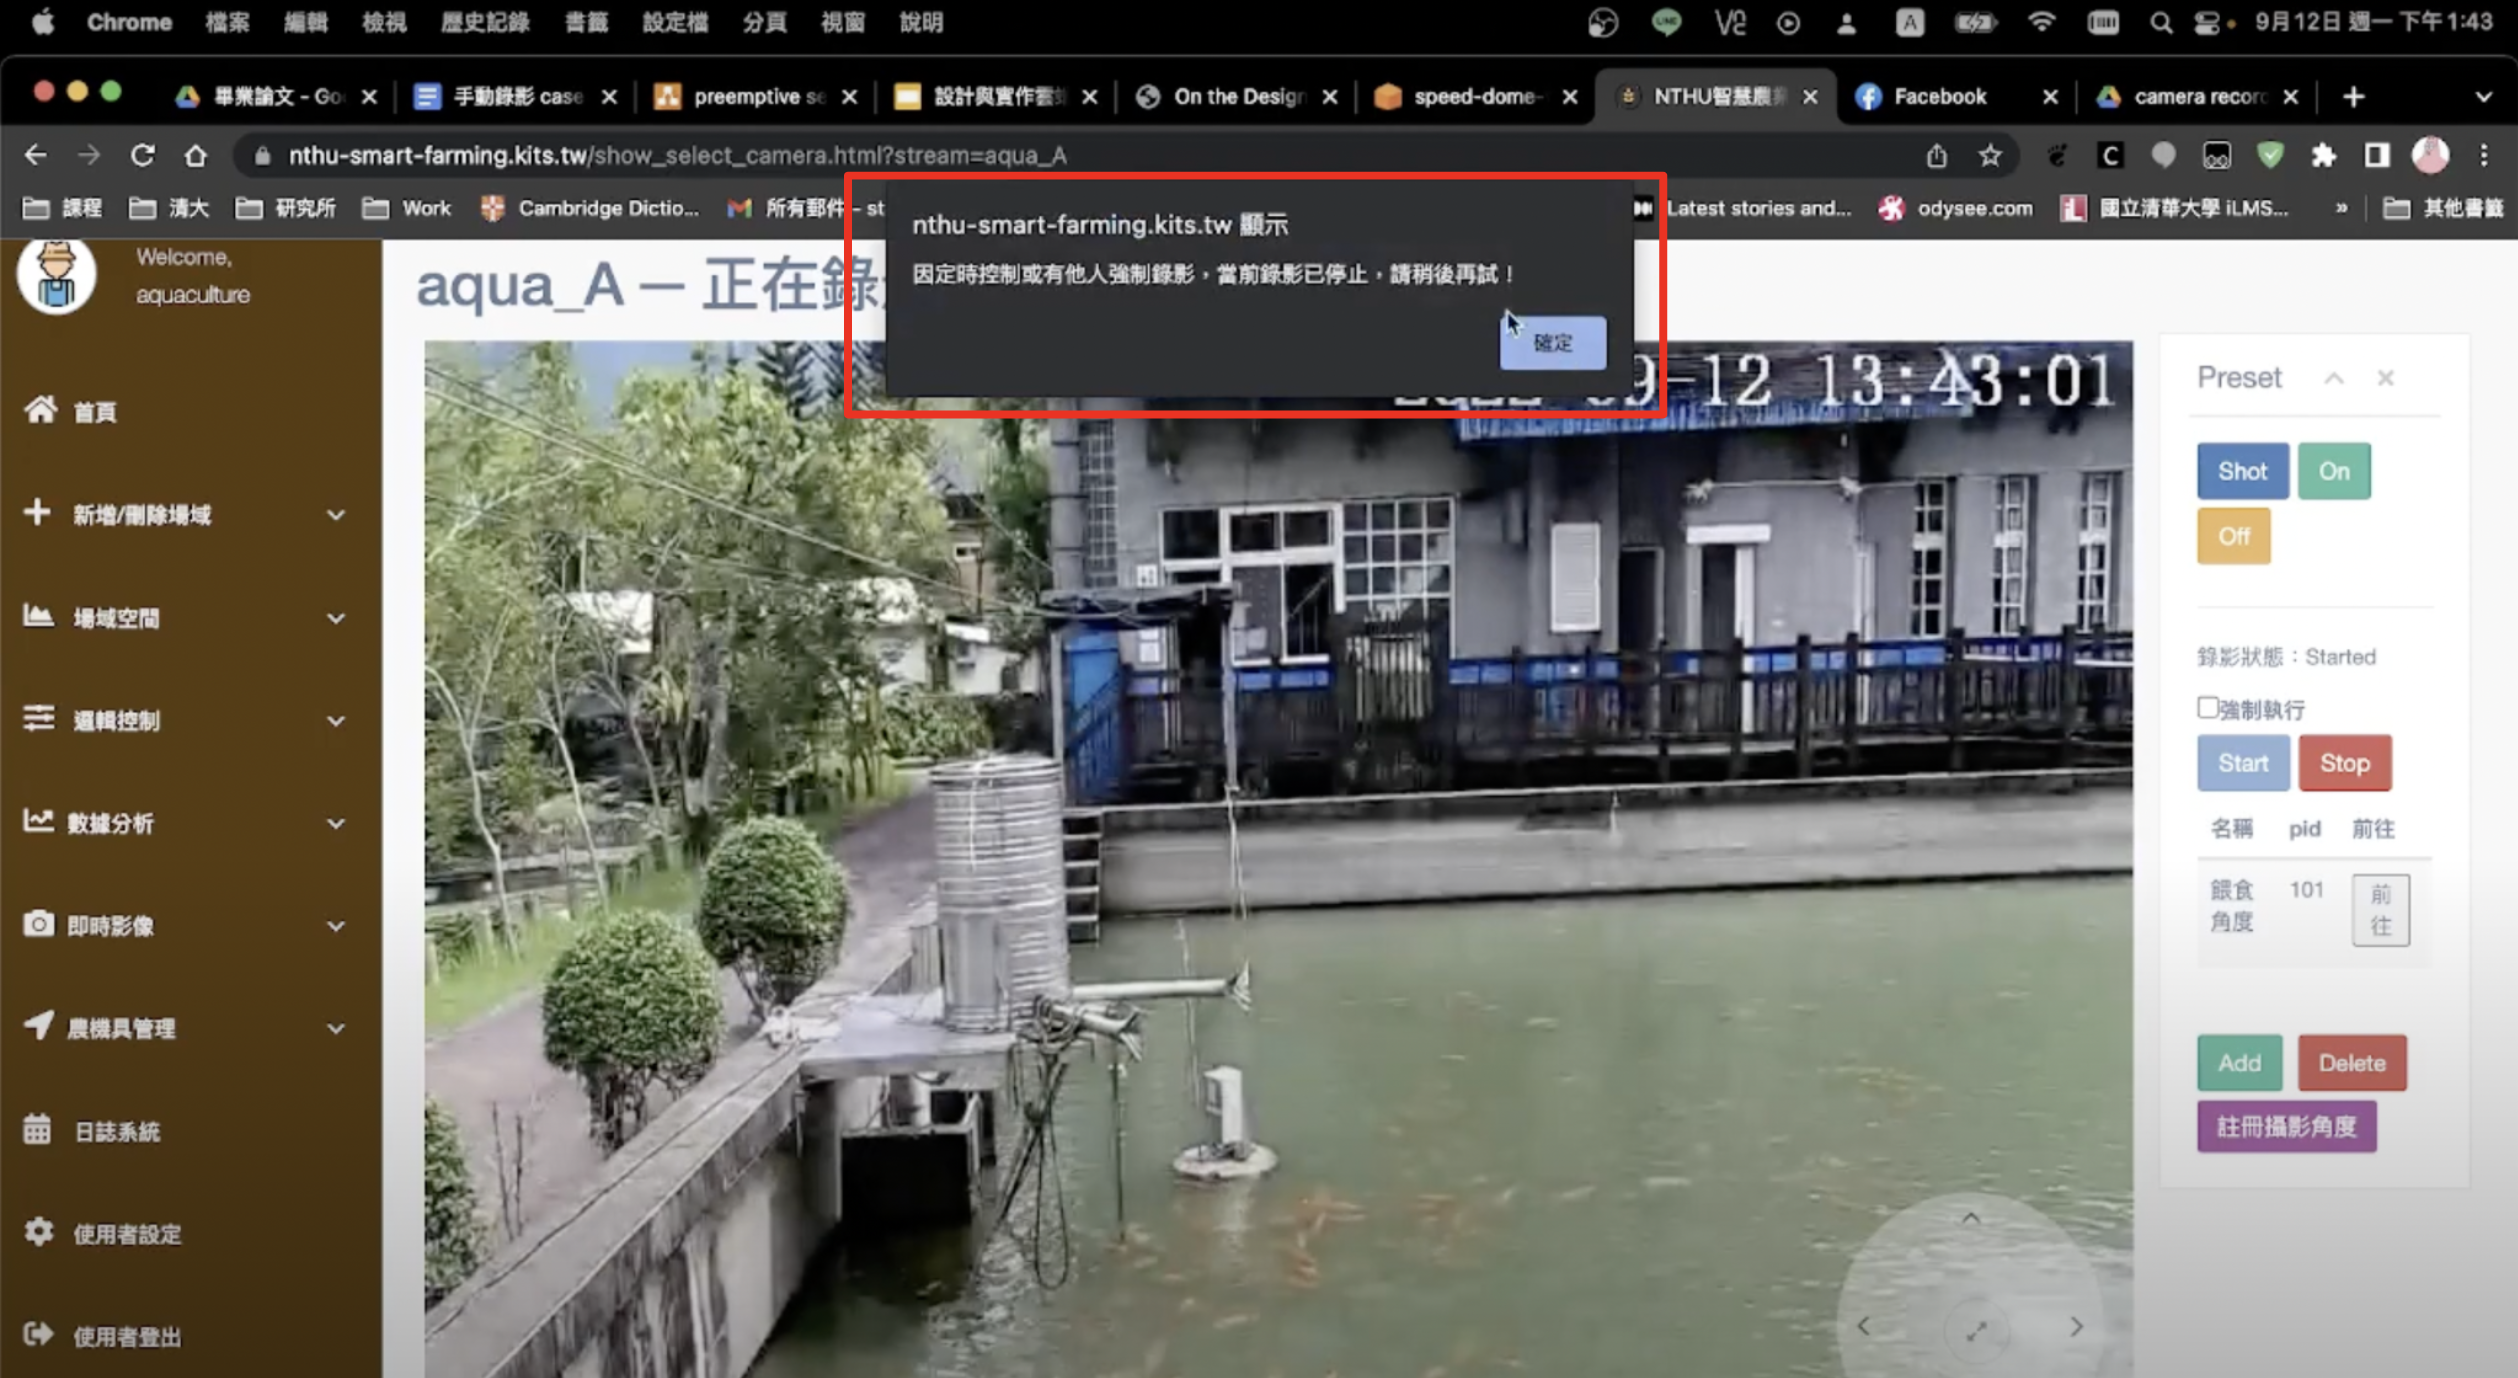
\includegraphics[width=\textwidth]{figsrc/demo-higher-3.png}
        \subcaption{New task preempt old task}
        \label{fig:demo-higher-3}
    \end{subfigure}

    \caption{DEMO of higher preemptive case}
    \label{fig:demo-higher}
\end{figure}

\subsection{Lower preemptive case}
Video DEMO: https://www.youtube.com/watch?v=1SY6WzD8WKA

We will show how higher priority task preempt lower priority one in Front-end perspective. In Fig.~\ref{fig:demo-lower-1}, we use two web page to simulate two manual recording request. Leftside of the web page will execute with higher priority by pressing forcing executing button at left down corner. In Fig.~\ref{fig:demo-lower-2}, right side user gets rejection when left side user is occupying the resource since its priority is lower than left side user.

\begin{figure}[H]
    \centering
    \begin{subfigure}{\textwidth}
        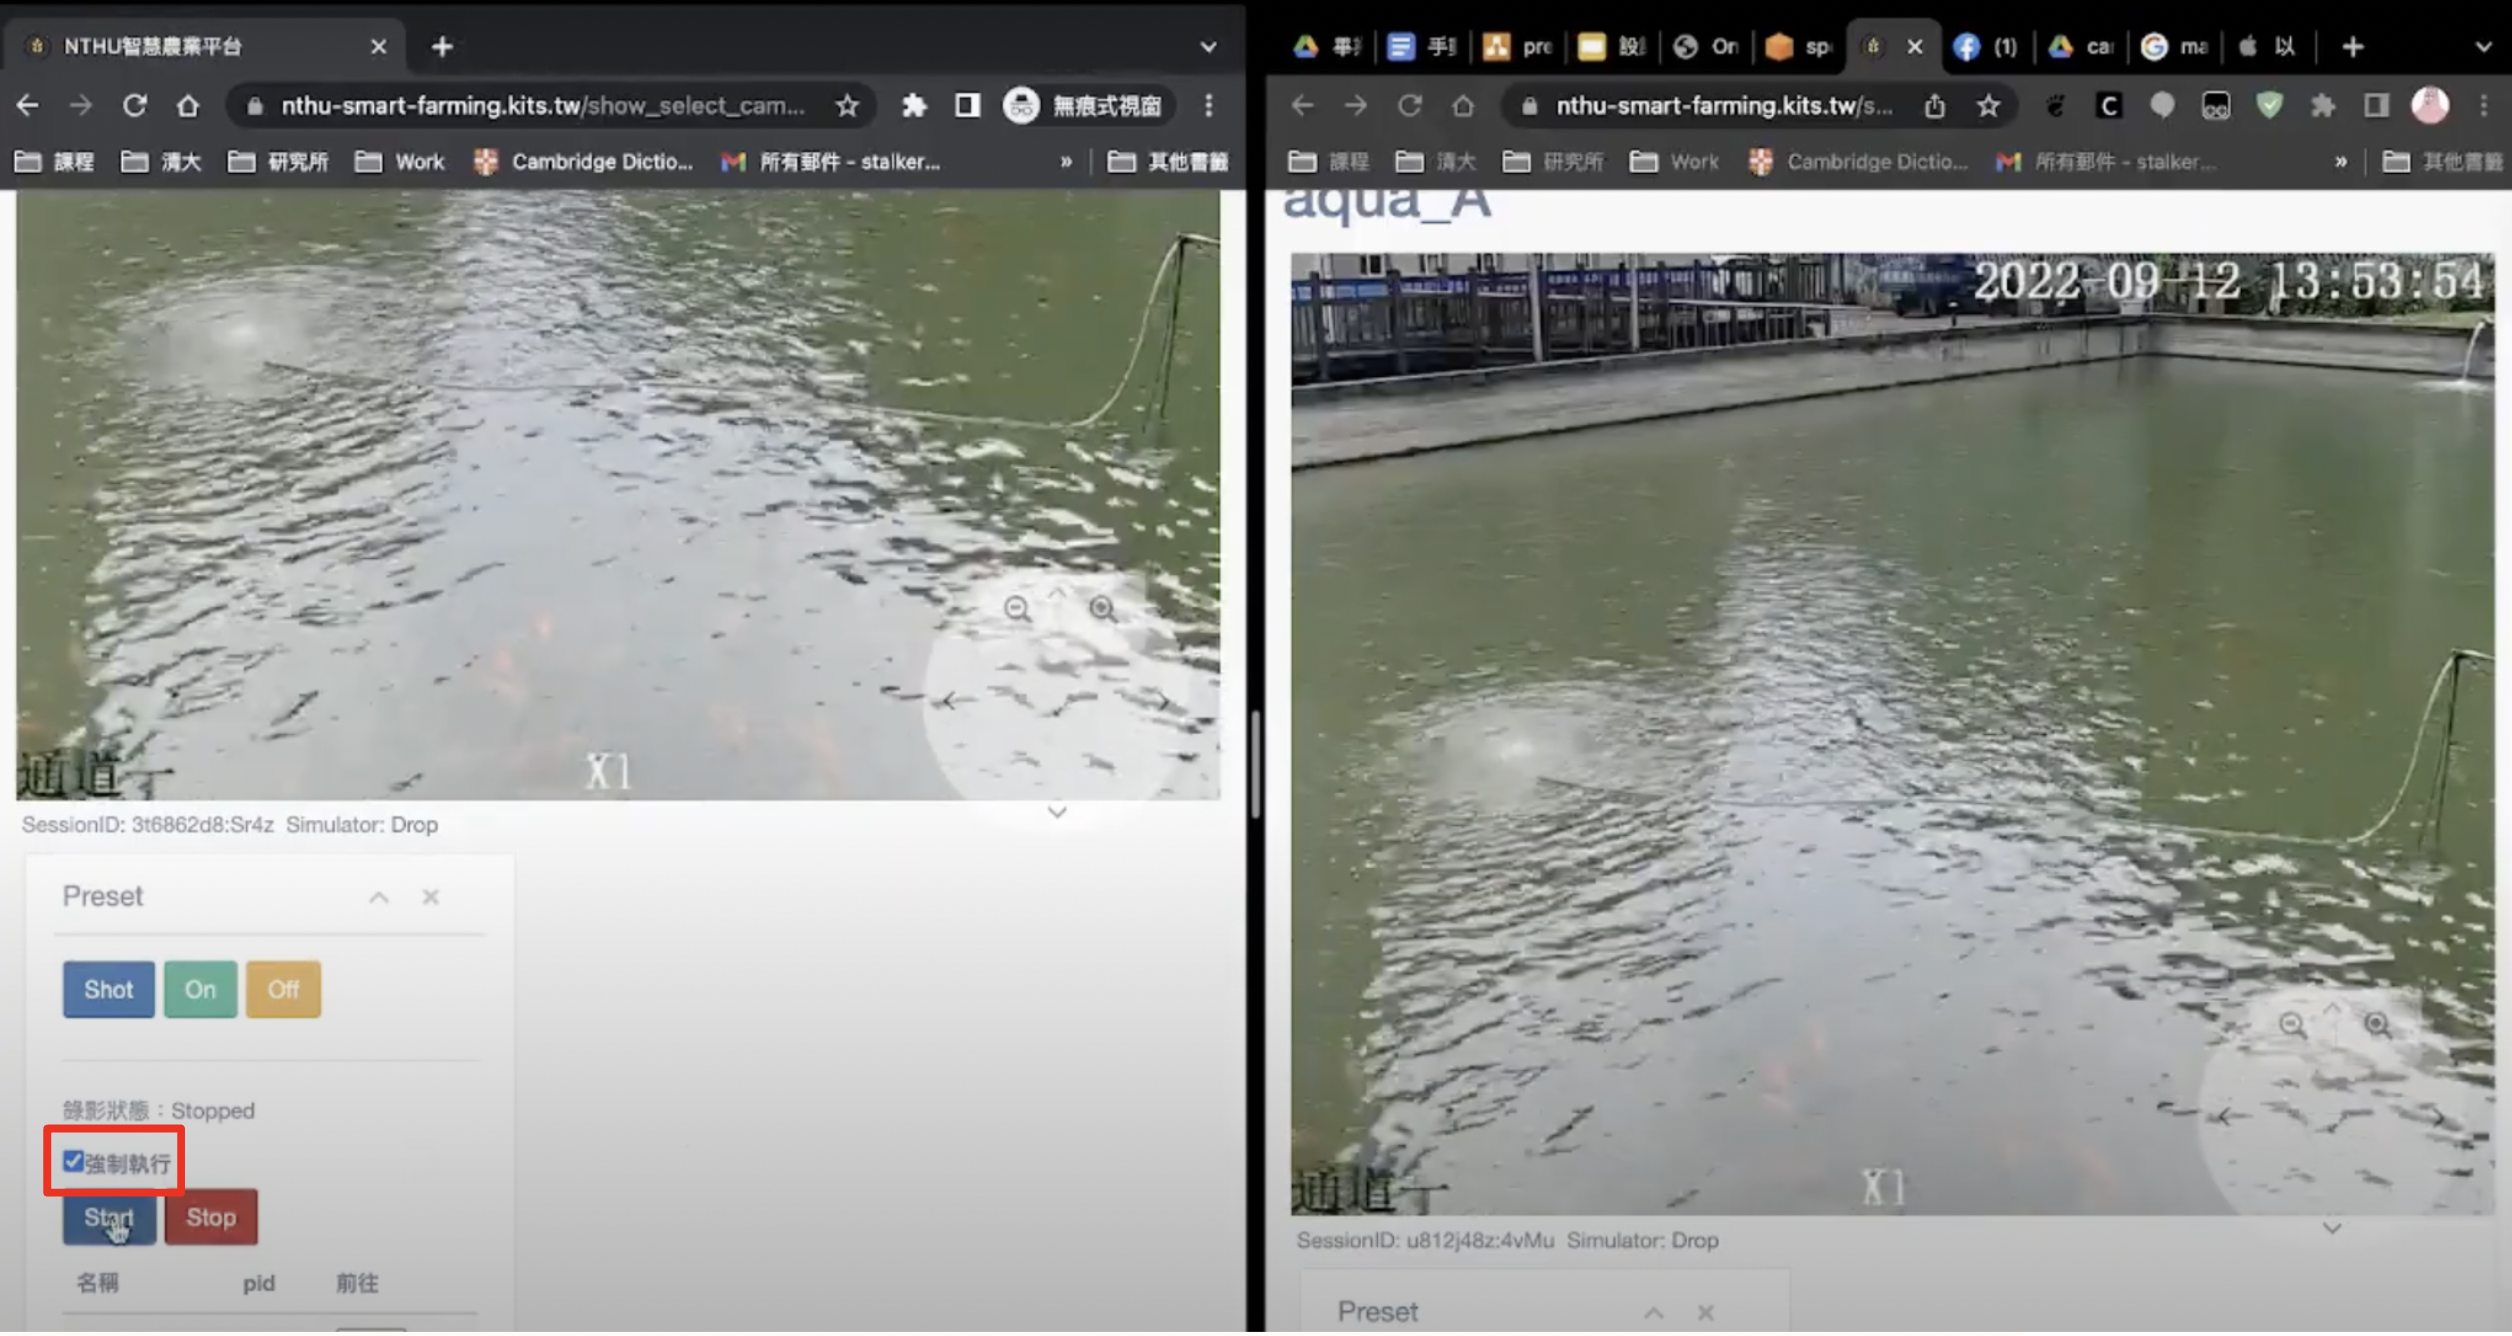
\includegraphics[width=\textwidth]{figsrc/demo-lower-1.png}
        \subcaption{Start with higher priority record at left side web page}
        \label{fig:demo-lower-1}
    \end{subfigure}
\end{figure}

\begin{figure}[H]
    \ContinuedFloat
    \centering
    \begin{subfigure}{\textwidth}
        \includegraphics[width=\textwidth]{figsrc/demo-lower-2.png}
        \subcaption{Right side user gets rejection while left side is recording}
        \label{fig:demo-lower-2}
    \end{subfigure}

    \caption{DEMO of lower rejection case}
    \label{fig:demo-lower}
\end{figure}

% 希望之後有像下面影片這樣的應用
% 單一工作效能分析 4階段
\section{Experiment Results}
Here we will measure our system performance. We divide the whole recording process into 4 phases, including permission request, build connection, recording and uploading as shown in Fig.~\ref{fig:result-4phases}. If we don't count preemptive case, we have three major use cases, manual, time period and event trigger. We use manual case to analyze the performance of the system. Because other two cases only have 3 phases, build connection, recording and uploading. They don't have permission request phase.

\begin{figure}[H]
    \centering
    \includegraphics[width=\textwidth]{figsrc/result-4phases.png}
    \caption{4 phases in manual cases\label{fig:result-4phases}}
\end{figure}

% pre
\subsection{Phase 1: Permission request}
In Permission request phase, PI will check whether the user have permission or not. We will measure the time elapsed from http request to http response. We send http request 500 times then get the latency chart below in Fig.~\ref{fig:result-p1}. We can see that the average time elapsed for requesting permission is 902.856ms and STD is 308.034.

\begin{figure}[H]
    \centering
    \includegraphics[width=\textwidth]{figsrc/result-p1.png}
    \caption{Latency of requesting permission over 500 times\label{fig:result-p1}}
\end{figure}

% build
\subsection{Phase 2: Build connection}
In build connection phase, we will measure the time from start sending MQTT recording command until recording server repsonds that it completes connection to streaming server as shown in Fig.~\ref{fig:result-p2-1}. Because recording command and reponse are both sent by MQTT, we use a local device to measure the time elapsed as shown in Fig.~\ref{fig:result-p2-2}. We will subtract the beginning time from the ending time to obtain latency. we repeat the experiment 200 times and each test has 1 minute interval. As shown in Fig.~\ref{fig:result-p2-3}, We see that average time elasped is 6408ms anf STD is 202. 

\begin{figure}[H]
    \centering
    \includegraphics[width=\textwidth]{figsrc/result-p2-1.png}
    \caption{Starting point and ending point of phase 2 latency\label{fig:result-p2-1}}
\end{figure}

\begin{figure}[H]
    \centering
    \includegraphics[width=\textwidth]{figsrc/result-p2-2.png}
    \caption{Get the MQTT message from 2 server then measure the time elapsed\label{fig:result-p2-2}}
\end{figure}

% result-p2-3
\begin{figure}[H]
    \centering
    \includegraphics[width=\textwidth]{figsrc/result-p2-3.png}
    \caption{Latency of building connection\label{fig:result-p2-3}}
\end{figure}

% recording
\subsection{Phase 3: Recording}
We will ignore the recording phase since the latency is determined by how long the recording process takes.

% uplaod
\subsection{Phase 4: Uploading}
In uploading phase, we measure the latency by the network bandwith since our recording server is deployed in AWS EC2. The time elasped of uploading phase is detemined by the recording duration, or size of video file. Thus, we will determine our time elapsed by measuring how many MB can be sent per second(i.e how fast is the network bandwidth of AWS EC2). The video SPEC has resolution of 1920x1080, 15 FPS and video duration of 300s. The video file size is about 495MB. We repeat the experiment for 50 times. As shown in Fig.~\ref{fig:result-p4-1}, the average upload time is 7583ms. In other words, the bandwidth of AWS EC2 is 73.637MB per second or we can say that it takes average 25.277ms to upload every 1 second of video.

\begin{figure}[H]
    \centering
    \includegraphics[width=\textwidth]{figsrc/result-p4-1.png}
    \caption{Latency of uploading\label{fig:result-p4-1}}
\end{figure}

\subsection{Observation}
Phase 1 has average delay of 902.856ms and Phase 2 has average delay of 6408ms. Phase 4 has average network bandwidth of 73.637MB/s. We can see that the bottleneck of the whole recording process is caused by building connection if the video file is small. But if the duration of video file exceeds 283s then upload time will be the bottleneck. As for user perspective, we expect that users concern more about the delay caused by Phase 1 + 2. So it may be better to improve the delay in Phase 1 + 2. Becuse it is usual that we care more about how long we have to wait to start the recording task.

\section{Scalability analysis}
We have shown the detail performance of single recording task. But what if there are multiple record tasks executing at the same time. Here we will show another bottleneck of the whole system. Recording process in recording server is the most resource-consuming task in the system. So we will test the performance of it by running different amount of tasks at the same time in recording server. As mentioned in Chapter 3, Our Recording server runs in AWS EC2. Operating System of EC2 VM is Ubuntu22.04. CPU is single Intel(R) Xeon(R) CPU E5-2676 v3 @ 2.40GH. RAM has size of 1 GB. As shown in Fig.~\ref{fig:result-scalability}, X-axis represents how many tasks are running at the same time. Y-axis represents the percentage of each components, such as Average CPU usage, Average RAM usage and Maximum CPU usage. Each number of task runs 5 times then calculate its average. We find that current server is only capable of running less than 5 task at the same time, if we don't want CPU usage exceed 70\% to make sure the stability of server. Although we have characteristic of automation and cloud-based in this system, scalability is what we need to improve in the future work.

\begin{figure}[H]
    \centering
    \includegraphics[width=\textwidth]{figsrc/result-scalability.png}
    \caption{Performance of multiple recording task\label{fig:result-scalability}}
\end{figure}

We also show the performace of phase 2 when they run different number of tasks at the same time in Fig.~\ref{fig:result-scale-2}. It shows that number of tasks running at the same time has little effect on phase 2. 

\begin{figure}[H]
    \centering
    \includegraphics[width=\textwidth]{figsrc/result-scale-2.png}
    \caption{\label{fig:result-scale-2}}
\end{figure}

% 總結比較
% 可擴充性問題

\chapter{Conclusion and future work}
\label{c:conclusion}




\if 0
\bibliography{thesis}
\graphicspath{{./figsrc/}}
\fi
% In this thesis, we proposed a recording streaming system which is efficient, automatic and cloud based. It can preset time scheduling for specific timing to record and register events to trigger record process when sonething critical happened. Also, we use AWS as our cloud service which improve storage limit, difficulty of maintaining system and developing new feature etc.. At last, We can manage all of the camera in experimental field located all over Taiwan.

In this thesis, we proposed an automatic, cloud-based and efficient system that was based on smart farming platform to collect video data for expert analysis or AI model training. We have shown in chapter 2 that there were many related recording streaming systems in the world. Although they had some advantage in their own product, it still didn't fit our requirements. Some products were lack of automation and others were lack of cloud support. Our system covered all of the user cases that we could think of, including user cases in other systems. To make the development more easier, we used some native services that were already existed in Smart farming platform(e.g. Video streaming server, Scheduling server etc.) then extent these to further implement new functions. We enumerated 3 user cases in our user scenarios, manual case, event triggered case and time triggered case. Addtionally, we even came out with a critical user scenario, preemptive user case. Based on these 3 + 1 cases, we implemented our core components, PI and recording server. To deal with preemptive case, we designed PI to make it able to decide which recording task should stay and which to terminate. Addtionally, PI also had the ability to communicate with recording server so that it could know what should do next. For recording server, we had shown that it was responsible of recieving command from PI, reporting server status to PI and executing recording task. To make system more reliable, we use AWS cloud service as our critical backbone. We use DynamoDB to store important meta data for camera and PI; Use S3 to store our video file; Use Greengrass and lambda to deploy our function in PI remotely; Use EC2 to run our recording server.

We have some improvement that can be done in the future. First, the delay time to build connection can be improved. Since it is important for user experience(UX) to not wait too long to start a recording process. Second, video quality can be improved. We can see in DEMO video that the streaming is obscure. Although the camera works fine in other field, we think that our camera is hard to focus on water surface. Third, recording server is capable of running multiple recording tasks at the same time but it cannot run too many. These may become issue if there are more than 5 tasks coming at the same time. Recording server needs a more scalable design.



% \input{discussion}
% \chapter{Conclusion and future work}
\label{c:conclusion}




\if 0
\bibliography{thesis}
\graphicspath{{./figsrc/}}
\fi
% In this thesis, we proposed a recording streaming system which is efficient, automatic and cloud based. It can preset time scheduling for specific timing to record and register events to trigger record process when sonething critical happened. Also, we use AWS as our cloud service which improve storage limit, difficulty of maintaining system and developing new feature etc.. At last, We can manage all of the camera in experimental field located all over Taiwan.

In this thesis, we proposed an automatic, cloud-based and efficient system that was based on smart farming platform to collect video data for expert analysis or AI model training. We have shown in chapter 2 that there were many related recording streaming systems in the world. Although they had some advantage in their own product, it still didn't fit our requirements. Some products were lack of automation and others were lack of cloud support. Our system covered all of the user cases that we could think of, including user cases in other systems. To make the development more easier, we used some native services that were already existed in Smart farming platform(e.g. Video streaming server, Scheduling server etc.) then extent these to further implement new functions. We enumerated 3 user cases in our user scenarios, manual case, event triggered case and time triggered case. Addtionally, we even came out with a critical user scenario, preemptive user case. Based on these 3 + 1 cases, we implemented our core components, PI and recording server. To deal with preemptive case, we designed PI to make it able to decide which recording task should stay and which to terminate. Addtionally, PI also had the ability to communicate with recording server so that it could know what should do next. For recording server, we had shown that it was responsible of recieving command from PI, reporting server status to PI and executing recording task. To make system more reliable, we use AWS cloud service as our critical backbone. We use DynamoDB to store important meta data for camera and PI; Use S3 to store our video file; Use Greengrass and lambda to deploy our function in PI remotely; Use EC2 to run our recording server.

We have some improvement that can be done in the future. First, the delay time to build connection can be improved. Since it is important for user experience(UX) to not wait too long to start a recording process. Second, video quality can be improved. We can see in DEMO video that the streaming is obscure. Although the camera works fine in other field, we think that our camera is hard to focus on water surface. Third, recording server is capable of running multiple recording tasks at the same time but it cannot run too many. These may become issue if there are more than 5 tasks coming at the same time. Recording server needs a more scalable design.



\appendix

\backmatter

\renewcommand{\bibname}{References}
\addcontentsline{toc}{chapter}{\bibname}
\bibliographystyle{ieeetr}

% Your bibliography goes here
{\singlespacing
 \bibliography{thesis}
}

\end{document}
